\chapterimage{Pictures/chap06/landscape-dof-960x1920.png}
\chapter{相机模型}\label{chap:相机模型}
\setcounter{sidenote}{1}

在第\refchap{绪论}中,我们介绍了计算机图形学中常用的针孔相机模型。
该模型很容易描述和模拟,但它忽略了真实相机中透镜对于穿过的光线具有的重要效应。
例如,针孔相机渲染的所有东西都是清晰对焦的——真实透镜系统不可能达到这种状态。
这样的图像常常看得出来是计算机生成的。
更一般地,离开透镜系统的辐射分布和进入它的分布有很大区别;
对透镜的这种效应建模对于准确模拟成像的辐射度量非常重要。

相机透镜系统也会引入各种影响其所构建图像的\keyindex{像差}{aberration}{};
例如,因为能到达胶片或传感器边缘的光比中心处更少,
\keyindex{暗角}{vignetting}{}\sidenote{译者注:也称晕影。}导致图像边缘变暗。
透镜也可以造成\keyindex{枕状畸变}{pincushion distortion}{distortion畸变}或\keyindex{桶状畸变}{barrel distortion}{distortion畸变},
即让直线成像为曲线。
尽管透镜设计者尽力在其设计中最小化像差,但它们仍可对图像有明显作用。

像第\refchap{形状}的\refvar{Shape}{}那样,pbrt中的相机也表示为抽象基类。
本章介绍类\refvar{Camera}{}及其两个关键方法\refvar[GenerateRay]{Camera::GenerateRay}{()}
和\refvar[GenerateRayDifferential]{Camera::GenerateRayDifferential}{()}。
第一个方法计算对应于胶片平面上样本位置的世界空间光线。
通过基于不同成像模型的不同方法生成这些光线,pbrt中的相机可以创建同一3D场景的多种图像。
第二种方法不仅生成该光线还计算采样该光线的图像区域的信息;
例如该信息用于第\refchap{纹理}的抗锯齿计算。
在\refsub{采样相机2}将介绍一些额外的\refvar{Camera}{}方法以支持双向光传输算法。

本章中,我们将展示\refvar{Camera}{}接口的一些实现,
从实现具有一定普遍性的理想针孔模型开始,
到和真实世界相机一样能模拟光穿过一组玻璃透镜元件成像的逼真模型结束。

\section{相机模型}\label{sec:相机模型}

\label{code:overview_Camera}
\begin{lstlisting}
`\initcode{Camera Declarations}{=}\initnext{CameraDeclarations}`
class Camera {
public:
    `\refcode{Camera Interface}{}`
    `\refcode{Camera Public Data}{}`
};
\end{lstlisting}

\section{投影相机模型}\label{sec:投影相机模型}

三维计算机图形学中的一个基本问题是{\itshape 3D视见问题}:
如何将三维场景投影到二维图像上进行显示。
大多数经典方法都可以用$4\times4$的\keyindex{投影变换}{projective transformation}{transformation变换}矩阵来表达。
因此,我们将引入一个投影矩阵相机类\refvar{ProjectiveCamera}{},
然后在此基础上定义两个相机模型。
第一个实现了\keyindex{正交投影}{orthographic projection}{projection投影},
另一个实现了\keyindex{透视投影}{perspective projection}{projection投影}——
两种经典且广泛使用的\keyindex{投影}{projection}{}。
\begin{lstlisting}
`\initcode{Camera Declarations}{+=}\lastcode{CameraDeclarations}`
class `\initvar{ProjectiveCamera}{}` : public `\refvar{Camera}{}` {
public:
    `\refcode{ProjectiveCamera Public Methods}{}`
protected:
    `\refcode{ProjectiveCamera Protected Data}{}`
};
\end{lstlisting}

还有三个坐标系(总结于\reffig{6.1}中)对定义和讨论投影相机很有用。
\begin{itemize}
    \item \keyindex{屏幕空间}{screen space}{}:
          屏幕空间定义在胶片平面上。相机将相机空间中的物体投影到胶片平面上;
          \keyindex{屏幕窗口}{screen window}{}内的部分在生成的图像中是可见的。
          屏幕空间的深度$z$值从0变到1,分别对应近处和远处截平面的点。
          注意,虽然这称为“屏幕”空间,但它仍然是一个三维坐标系,因为$z$值是有意义的。
    \item \keyindex{规范化设备坐标}{normalized device coordinate}{}(NDC){\sffamily 空间}:
          这是被渲染的实际图像的坐标系。对于$x$和$y$,该空间范围从$(0,0)$变到$(1,1)$,
          其中$(0,0)$是图像的左上角。深度值与屏幕空间中的相同,线性变换将屏幕空间转换为NDC空间。
    \item \keyindex{栅格空间}{raster space}{}\sidenote{译者注:也称光栅空间。}:
          这与NDC空间几乎相同,除了$x$和$y$坐标从$(0,0)$变到(resolution.x, resolution.y)
          \sidenote{译者注:resolution指分辨率。}。
\end{itemize}

投影相机用$4\times4$矩阵在所有这些空间之间进行转换,
但具有特殊成像特性的相机不必用矩阵表示所有这些转换。
\begin{figure}[htbp]
    \centering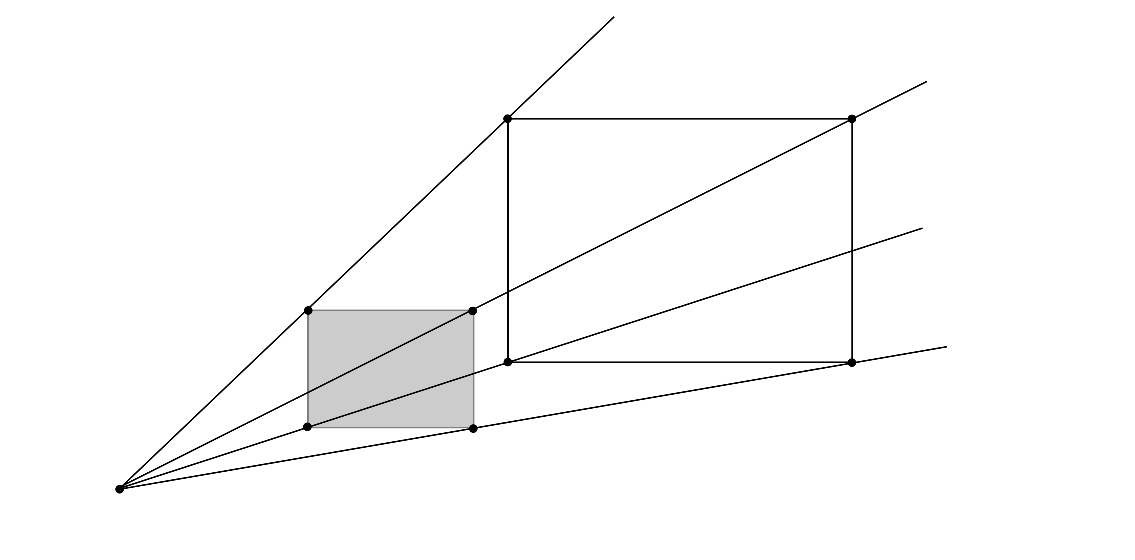
\includegraphics[width=0.75\linewidth]{chap06/Cameracoordinatespaces.eps}
    \put(-280,0){\small 相机空间:$(0,0,0)$}
    \put(-270,60){\small NDC:$(0,0,0)$}
    \put(-220,110){\small NDC:$(0,0,1)$}
    \put(-160,20){\small $z=\text{near}$}
    \put(-160,10){\small NDC:$(1,1,0)$}
    \put(-160,0){\small 栅格:$(\text{res}.x,\text{res}.y,0)$}
    \put(-70,35){\small $z=\text{far}$}
    \put(-70,25){\small NDC:$(1,1,1)$}
    \put(-70,15){\small 栅格:$(\text{res}.x,\text{res}.y,1)$}
    \caption{几个与相机相关的坐标空间常用于简化\protect\refvar{Camera}{}的实现。
        相机类持有它们之间的变换。世界空间中的场景物体由相机查看,它位于相机空间原点,并指向$+z$轴。
        近处和远处平面之间的物体被投影到相机空间中的胶片平面$z=\text{near}$上。
        胶片平面在栅格空间中$z=0$处,其中$x$和$y$范围从$(0,0)$变到(resolution.x, resolution.y)。
        规范化设备坐标(NDC)空间将栅格空间归一化,因此$x$和$y$范围从$(0,0)$变到$(1,1)$。}
    \label{fig:6.1}
\end{figure}

除了基类\refvar{Camera}{}要求的参数外,\refvar{ProjectiveCamera}{}还接收投影变换矩阵、
图像的屏幕空间范围以及与景深有关的额外参数。
\keyindex{景深}{depth of field}{}将在本节末尾介绍和实现,
它模拟了真实透镜系统中出现的失焦物体的模糊性。
\begin{lstlisting}
`\initcode{ProjectiveCamera Public Methods}{=}`
`\refvar{ProjectiveCamera}{}`(const `\refvar{AnimatedTransform}{}` &CameraToWorld, 
        const `\refvar{Transform}{}` &CameraToScreen, const `\refvar{Bounds2f}{}` &screenWindow,
        `\refvar{Float}{}` shutterOpen, `\refvar{Float}{}` shutterClose, `\refvar{Float}{}` lensr, `\refvar{Float}{}` focald,
        `\refvar{Film}{}` *film, const `\refvar{Medium}{}` *medium)
    : `\refvar{Camera}{}`(CameraToWorld, shutterOpen, shutterClose, film, medium),
      `\refvar{CameraToScreen}{}`(CameraToScreen) {
    `\refcode{Initialize depth of field parameters}{}`
    `\refcode{Compute projective camera transformations}{}`
}
\end{lstlisting}

\refvar{ProjectiveCamera}{}的实现将投影变换传递给这里展示的基类构造函数。
该变换给出了相机到屏幕的投影;
由此,构造函数能轻松算出从栅格空间到相机空间一路所需的其他变换。
\begin{lstlisting}
`\initcode{Compute projective camera transformations}{=}`
`\refcode{Compute projective camera screen transformations}{}`
`\refvar{RasterToCamera}{}` = `\refvar[Transform::Inverse]{Inverse}{}`(CameraToScreen) * `\refvar{RasterToScreen}{}`;
\end{lstlisting}
\begin{lstlisting}
`\initcode{ProjectiveCamera Protected Data}{=}\initnext{ProjectiveCameraProtectedData}`
`\refvar{Transform}{}` `\initvar{CameraToScreen}{}`, `\initvar{RasterToCamera}{}`;
\end{lstlisting}

在构造函数中唯一要计算的重要变换是屏幕到栅格的投影。
在下面的代码中,请注意变换的组成(从下往上看),
我们从屏幕空间的一个点开始,先平移使得屏幕左上角位于原点,
然后用屏幕宽度和高度的倒数进行缩放,
得到一个$x$和$y$坐标在0到1之间的点(这些是NDC坐标)。
最后,我们用栅格化分辨率进行缩放,这样我们最终就能完全覆盖
从$(0,0)$直到整个栅格分辨率的栅格范围。
这里一个重要细节是$y$坐标被该变换倒置了;
这是必要的,因为增加的$y$值在屏幕坐标中是向上移动但在栅格坐标中是向下的。
\begin{lstlisting}
`\initcode{Compute projective camera screen transformations}{=}`
`\refvar{ScreenToRaster}{}` = `\refvar{Scale}{}`(film->`\refvar{fullResolution}{}`.x, 
                       film->`\refvar{fullResolution}{}`.y, 1) *
    `\refvar{Scale}{}`(1 / (screenWindow.`\refvar{pMax}{}`.x - screenWindow.`\refvar{pMin}{}`.x),
          1 / (screenWindow.`\refvar{pMin}{}`.y - screenWindow.`\refvar{pMax}{}`.y), 1) *
    `\refvar{Translate}{}`(`\refvar{Vector3f}{}`(-screenWindow.`\refvar{pMin}{}`.x, -screenWindow.`\refvar{pMax}{}`.y, 0));
`\refvar{RasterToScreen}{}` = `\refvar[Transform::Inverse]{Inverse}{}`(`\refvar{ScreenToRaster}{}`);
\end{lstlisting}
\begin{lstlisting}
`\refcode{ProjectiveCamera Protected Data}{+=}\lastnext{ProjectiveCameraProtectedData}`
`\refvar{Transform}{}` `\initvar{ScreenToRaster}{}`, `\initvar{RasterToScreen}{}`;
\end{lstlisting}

\subsection{正交相机}\label{sub:正交相机}
\begin{lstlisting}
`\initcode{OrthographicCamera Declarations}{=}`
class `\initvar{OrthographicCamera}{}` : public `\refvar{ProjectiveCamera}{}` {
public:
    `\refcode{OrthographicCamera Public Methods}{}`
private:
    `\refcode{OrthographicCamera Private Data}{}`
};
\end{lstlisting}

定义在文件\href{https://github.com/mmp/pbrt-v3/blob/master/src/cameras/orthographic.h}{\ttfamily cameras/orthographic.h}和
\href{https://github.com/mmp/pbrt-v3/tree/master/src/cameras/orthographic.cpp}{\ttfamily cameras/orthographic.cpp}中的\keyindex{正交相机}{orthographic camera}{camera相机},
是基于正交投影变换的。
正交变换取场景中的一块矩形区域并将其投影到定义该区域之框的前方一面。
它不具有\keyindex{前缩}{foreshortening}{}效应——当物体远离时它们在成像平面上变小——
但它让平行线依然平行,并保留物体间的相对距离。
\reffig{6.2}{}展示了该立方体是如何定义场景可见区域的。
\begin{figure}[htbp]
    \centering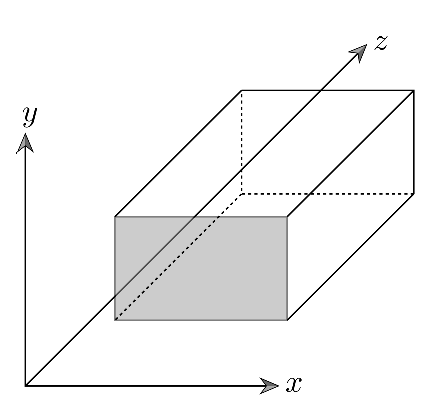
\includegraphics[width=0.33\linewidth]{chap06/Orthoviewingvolume.eps}
    \caption{正交视见体是相机空间中的轴对齐框,
        其定义使该区域内的物体投影到该框$z=\text{near}$的一面上。}
    \label{fig:6.2}
\end{figure}

\reffig{6.3}比较了用正交投影和下节定义的透视投影来渲染的结果
\sidenote{译者注:原图为exr格式,此处转换为png格式以便制作插图,
    图像细节和色域可能发生细微变化。后续均作此处理,读者可到原书官网查看原图。}。
\begin{figure}[htbp]
    \centering
    \subfloat[正交]{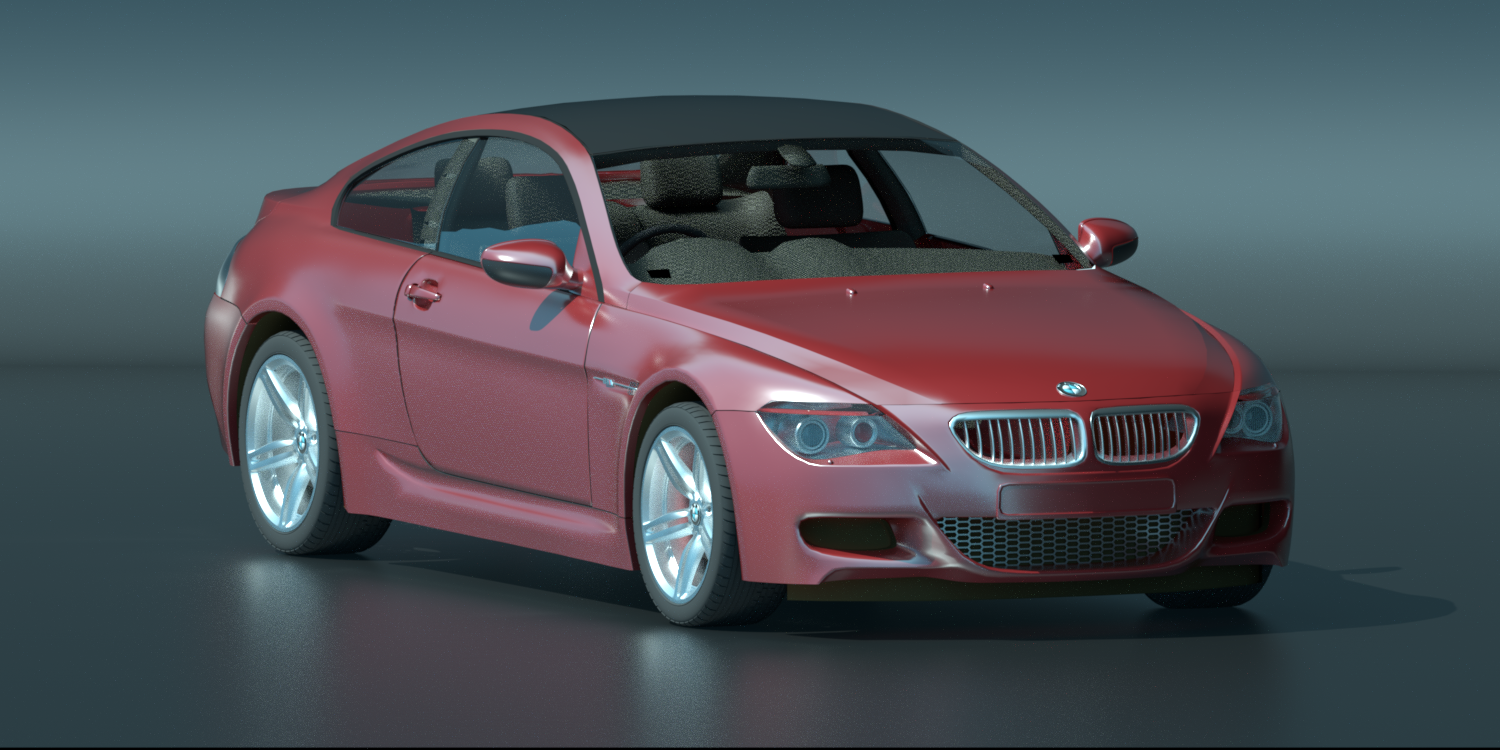
\includegraphics[width=\linewidth]{chap06/car-ortho.png}\label{fig:6.3.1}}\\
    \subfloat[透视]{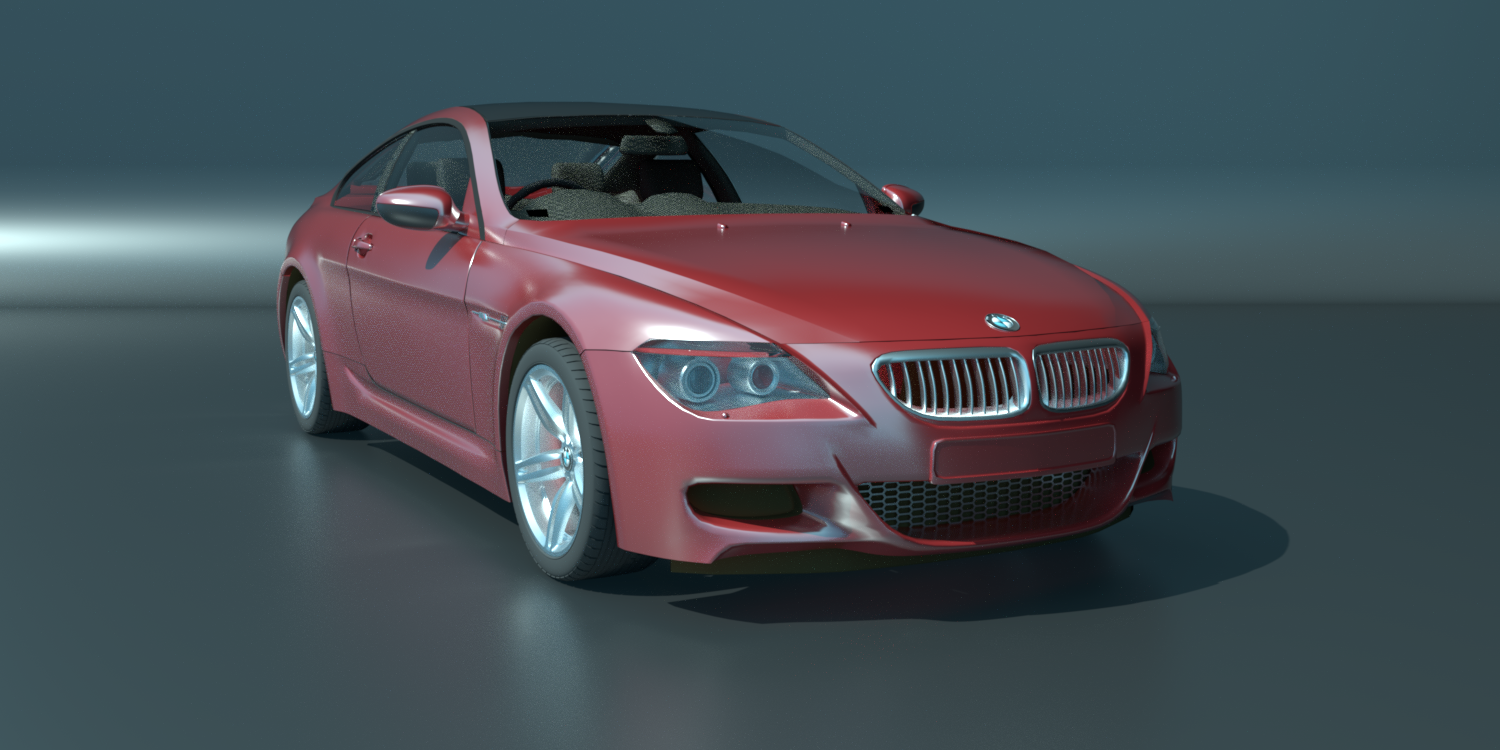
\includegraphics[width=\linewidth]{chap06/car-perspective.png}\label{fig:6.3.2}}
    \caption{用不同相机模型渲染的汽车模型。用(a)正交和(b)透视相机从同一视点渲染汽车。
        缺少前缩使得正交视角看起来深度更少,但它保留了平行线,是很有用的特性。}
    \label{fig:6.3}
\end{figure}

正交相机构造函数用稍后定义的函数\refvar{Orthographic}{()}生成正交变换矩阵。
\begin{lstlisting}
`\initcode{OrthographicCamera Public Methods}{=}`
`\refvar{OrthographicCamera}{}`(const `\refvar{AnimatedTransform}{}` &CameraToWorld,
        const `\refvar{Bounds2f}{}` &screenWindow, `\refvar{Float}{}` shutterOpen,
        `\refvar{Float}{}` shutterClose, `\refvar{Float}{}` lensRadius, `\refvar{Float}{}` focalDistance,
        `\refvar{Film}{}` *film, const `\refvar{Medium}{}` *medium)
    : `\refvar{ProjectiveCamera}{}`(CameraToWorld, `\refvar{Orthographic}{}`(0, 1),
                       screenWindow, shutterOpen, shutterClose,
                       lensRadius, focalDistance, film, medium) {
    `\refcode{Compute differential changes in origin for orthographic camera rays}{}`
}
\end{lstlisting}

正交视角变换保持$x$和$y$坐标不变但将近处平面的$z$值映射为0而远处平面的$z$值映射为1。
为此,场景先沿$z$轴平移使得近处平面对齐到$z=0$。
然后,场景按$z$缩放使得远处平面映射为$z=1$。
这两个变换合成得到整个变换。(对于像pbrt那样的光线追踪器,
我们想让近处平面位于0处,这样光线就会从穿过相机位置的平面上发出;
远处平面偏移量不是很重要。)
\begin{lstlisting}
`\refcode{Transform Method Definitions}{+=}\lastnext{TransformMethodDefinitions}`
`\refvar{Transform}{}` `\initvar{Orthographic}{}`(`\refvar{Float}{}` zNear, `\refvar{Float}{}` zFar) {
    return `\refvar{Scale}{}`(1, 1, 1 / (zFar - zNear)) *
           `\refvar{Translate}{}`(`\refvar{Vector3f}{}`(0, 0, -zNear));
}
\end{lstlisting}

幸亏正交投影很简单,在方法\refvar[OrthographicCamera::GenerateRayDifferential]{GenerateRayDifferential}{()}中
很容易直接计算$x$和$y$方向的差分射线。
差分射线的方向将和主射线一样(它们对于一个正交相机生成的所有光线都是这样),
且端点差异对于所有射线也会一样。
因此,这里的构造函数预先计算射线端点因胶片平面上在$x$和$y$方向移动单个像素而
在相机空间坐标中移动了多少。
\begin{lstlisting}
`\initcode{Compute differential changes in origin for orthographic camera rays}{=}`
`\refvar[OrthographicCamera::dxCamera]{dxCamera}{}` = `\refvar{RasterToCamera}{}`(`\refvar{Vector3f}{}`(1, 0, 0));
`\refvar[OrthographicCamera::dyCamera]{dyCamera}{}` = `\refvar{RasterToCamera}{}`(`\refvar{Vector3f}{}`(0, 1, 0));
\end{lstlisting}
\begin{lstlisting}
`\initcode{OrthographicCamera Private Data}{=}`
`\refvar{Vector3f}{}` `\initvar[OrthographicCamera::dxCamera]{dxCamera}{}`, `\initvar[OrthographicCamera::dyCamera]{dyCamera}{}`;
\end{lstlisting}

我们现在可以执行代码取栅格空间中的一个样本点并将其变为相机光线。
\reffig{6.4}总结了该过程。首先,栅格空间样本位置变换为相机空间的一点,
即给出近处平面上一点作为相机光线的端点。
因为相机空间观察方向沿$z$轴指出,相机空间光线方向为$(0,0,1)$。

\begin{figure}[htbp]
    \centering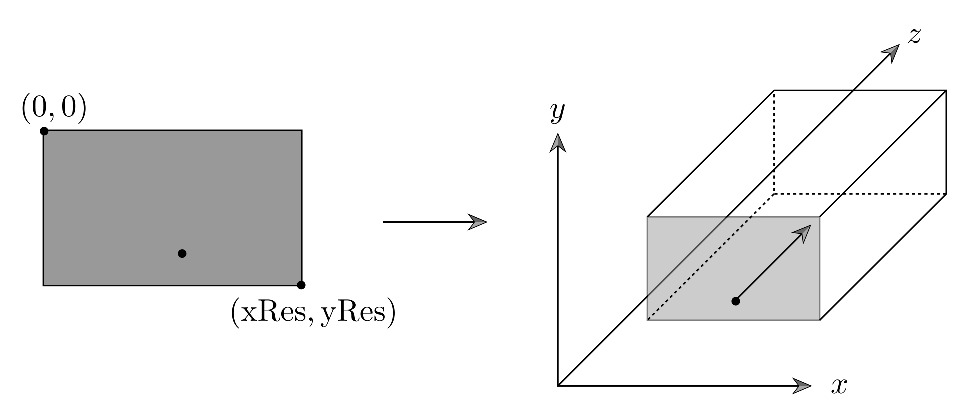
\includegraphics[width=0.8\linewidth]{chap06/Orthogenerateray.eps}
    \caption{为了用正交相机创建光线,胶片平面上的栅格空间位置被变换到相机空间,
        给出近处平面上的射线端点。相机空间中光线的方向为$(0,0,1)$,沿$z$轴。}
    \label{fig:6.4}
\end{figure}

若为该场景启用景深,则修改射线端点和方向来模拟景深。本节将稍后解释景深。
光线的时间值通过按偏移量\refvar{CameraSample::time}{}(在范围$[0,1)$内)
在快门开启和关闭间线性插值来设置。最后,光线在被返回前变换到世界空间。
\begin{lstlisting}
`\initcode{OrthographicCamera Definitions}{=}\initnext{OrthographicCameraDefinitions}`
`\refvar{Float}{}` `\refvar{OrthographicCamera}{}`::`\initvar[OrthographicCamera::GenerateRay]{\refvar{GenerateRay}{}}{}`(const `\refvar{CameraSample}{}` &sample,
        `\refvar{Ray}{}` *ray) const {
    `\refcode{Compute raster and camera sample positions}{}`
    *ray = `\refvar{Ray}{}`(pCamera, `\refvar{Vector3f}{}`(0, 0, 1));
    `\refcode{Modify ray for depth of field}{}`
    ray->`\refvar[Ray::time]{time}{}` = `\refvar{Lerp}{}`(sample.`\refvar[CameraSample::time]{time}{}`, `\refvar{shutterOpen}{}`, `\refvar{shutterClose}{}`);
    ray->`\refvar[Ray::medium]{medium}{}` = `\refvar[Camera::medium]{medium}{}`;
    *ray = `\refvar{CameraToWorld}{}`(*ray);
    return 1;
}
\end{lstlisting}

一旦设置好所有变换矩阵,就很容易将栅格空间样本变换到相机空间。
\begin{lstlisting}
`\initcode{Compute raster and camera sample positions}{=}`
`\refvar{Point3f}{}` pFilm = `\refvar{Point3f}{}`(sample.`\refvar{pFilm}{}`.x, sample.`\refvar{pFilm}{}`.y, 0);
`\refvar{Point3f}{}` pCamera = `\refvar{RasterToCamera}{}`(pFilm);
\end{lstlisting}

\refvar[OrthographicCamera::GenerateRayDifferential]{GenerateRayDifferential}{()}的实现执行一样的计算来生成相机主光线。
差分射线端点用在\refvar{OrthographicCamera}{}构造函数中算得的偏移量求出,
然后将整个射线差分变换到世界空间。
\begin{lstlisting}
`\refcode{OrthographicCamera Definitions}{+=}\lastcode{OrthographicCameraDefinitions}`
`\refvar{Float}{}` `\refvar{OrthographicCamera}{}`::`\initvar[OrthographicCamera::GenerateRayDifferential]{\refvar{GenerateRayDifferential}{}}{}`(
        const `\refvar{CameraSample}{}` &sample, `\refvar{RayDifferential}{}` *ray) const {
    `\refcode{Compute main orthographic viewing ray}{}`
    `\refcode{Compute ray differentials for OrthographicCamera}{}`
    ray->`\refvar[Ray::time]{time}{}` = `\refvar{Lerp}{}`(sample.`\refvar[CameraSample::time]{time}{}`, `\refvar{shutterOpen}{}`, `\refvar{shutterClose}{}`);
    ray->`\refvar{hasDifferentials}{}` = true;
    ray->`\refvar[Ray::medium]{medium}{}` = `\refvar[Camera::medium]{medium}{}`;
    *ray = `\refvar{CameraToWorld}{}`(*ray);
    return 1;
}
\end{lstlisting}
\begin{lstlisting}
`\initcode{Compute main orthographic viewing ray}{=}`
`\refcode{Compute raster and camera sample positions}{}`
*ray = `\refvar{RayDifferential}{}`(pCamera, `\refvar{Vector3f}{}`(0, 0, 1));
`\refcode{Modify ray for depth of field}{}`
\end{lstlisting}
\begin{lstlisting}
`\initcode{Compute ray differentials for OrthographicCamera}{=}`
if (`\refvar{lensRadius}{}` > 0) {
    `\refcode{Compute OrthographicCamera ray differentials accounting for lens}{}`
} else {
    ray->`\refvar{rxOrigin}{}` = ray->`\refvar[Ray::o]{o}{}` + `\refvar[OrthographicCamera::dxCamera]{dxCamera}{}`;
    ray->`\refvar{ryOrigin}{}` = ray->`\refvar[Ray::o]{o}{}` + `\refvar[OrthographicCamera::dyCamera]{dyCamera}{}`;
    ray->`\refvar{rxDirection}{}` = ray->`\refvar{ryDirection}{}` = ray->`\refvar[Ray::d]{d}{}`;
}
\end{lstlisting}
\begin{lstlisting}
`\initcode{Compute OrthographicCamera ray differentials accounting for lens}{=}`
`\refcode{Sample point on lens}{}`
`\refvar{Float}{}` ft = focalDistance / ray->`\refvar[Ray::d]{d}{}`.z;

`\refvar{Point3f}{}` pFocus = pCamera + `\refvar[OrthographicCamera::dxCamera]{dxCamera}{}` + (ft * `\refvar{Vector3f}{}`(0, 0, 1));
ray->`\refvar{rxOrigin}{}` = `\refvar{Point3f}{}`(pLens.x, pLens.y, 0);
ray->`\refvar{rxDirection}{}` = `\refvar{Normalize}{}`(pFocus - ray->`\refvar{rxOrigin}{}`);

pFocus = pCamera + `\refvar[OrthographicCamera::dyCamera]{dyCamera}{}` + (ft * `\refvar{Vector3f}{}`(0, 0, 1));
ray->`\refvar{ryOrigin}{}` = `\refvar{Point3f}{}`(pLens.x, pLens.y, 0);
ray->`\refvar{ryDirection}{}` = `\refvar{Normalize}{}`(pFocus - ray->`\refvar{ryOrigin}{}`);
\end{lstlisting}

\subsection{透视相机}\label{sub:透视相机}
透视投影和正交投影相似,也把一个空间体投影到2D胶片平面上。
然而,它包含前缩效应:远处物体比近处相同尺寸的物体投影得更小。
不像正交投影那样,透视投影不保持距离和角度,平行线也不再保持平行。
透视投影非常符合眼睛或相机透镜生成3D世界图像的方式。
投影相机实现于文件\href{https://github.com/mmp/pbrt-v3/blob/master/src/cameras/perspective.h}{\ttfamily cameras/perspective.h}
和\href{https://github.com/mmp/pbrt-v3/blob/master/src/cameras/perspective.cpp}{\ttfamily cameras/perspective.cpp}中。
\begin{lstlisting}
`\initcode{PerspectiveCamera Declarations}{=}`
class `\initvar{PerspectiveCamera}{}` : public `\refvar{ProjectiveCamera}{}` {
public:
    `\refcode{PerspectiveCamera Public Methods}{}`
private:
    `\refcode{PerspectiveCamera Private Data}{}`
};
\end{lstlisting}
\begin{lstlisting}
`\initcode{PerspectiveCamera Method Definitions}{=}\initnext{PerspectiveCameraMethodDefinitions}`
`\refvar{PerspectiveCamera}{}`::`\refvar{PerspectiveCamera}{}`(
        const `\refvar{AnimatedTransform}{}` &CameraToWorld,
        const `\refvar{Bounds2f}{}` &screenWindow, `\refvar{Float}{}` shutterOpen,
        `\refvar{Float}{}` shutterClose, `\refvar{Float}{}` lensRadius, `\refvar{Float}{}` focalDistance,
        `\refvar{Float}{}` fov, `\refvar{Film}{}` *film, const `\refvar{Medium}{}` *medium)
    : `\refvar{ProjectiveCamera}{}`(CameraToWorld, `\refvar{Perspective}{}`(fov, 1e-2f, 1000.f),
                       screenWindow, shutterOpen, shutterClose,
                       lensRadius, focalDistance, film, medium) {
    `\refcode{Compute differential changes in origin for perspective camera rays}{}`
    `\refcode{Compute image plane bounds at z=1 for PerspectiveCamera}{}`
}
\end{lstlisting}

透视投影描述了场景的透视图。
场景中的点投影到垂直于$z$轴的视平面上。
函数\refvar{Perspective}{()}计算该变换;
它接收视场角度{\ttfamily fov}以及到近处$z$平面和远处$z$平面的距离。
在透视投影后,近处$z$平面上的点映射为$z=0$,远处平面上的点则有$z=1$(\reffig{6.5})。
对于基于栅格化的渲染系统,仔细设置这些平面的位置很重要;
它们决定了要渲染的场景的$z$范围,但将它们取值的量级设置得相差过大可能导致数值精度误差。
对于像pbrt的光线追踪器,可以按其位置任意设置它们。
\begin{figure}[htbp]
    \centering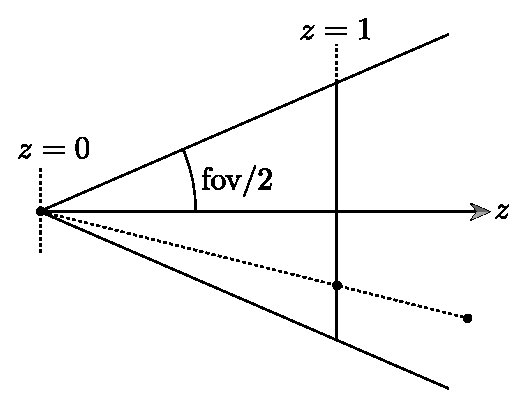
\includegraphics[width=0.5\linewidth]{chap06/Perspectivetransformationmatrix.eps}
    \caption{投影变换矩阵将相机空间里的点投影到胶片平面。
        被投影点的$x'$和$y'$坐标等于投影前$x$和$y$坐标除以$z$坐标。
        投影后的$z'$坐标的计算使得近处平面的点映射为$z'=0$而
        远处平面的点映射为$z'=1$。}
    \label{fig:6.5}
\end{figure}

\begin{lstlisting}
`\refcode{Transform Method Definitions}{+=}\lastcode{TransformMethodDefinitions}`
`\refvar{Transform}{}` `\initvar{Perspective}{}`(`\refvar{Float}{}` fov, `\refvar{Float}{}` n, `\refvar{Float}{}` f) {
    `\refcode{Perform projective divide for perspective projection}{}`
    `\refcode{Scale canonical perspective view to specified field of view}{}`
}
\end{lstlisting}
该变换最容易理解,分两个步骤:
\begin{enumerate}
    \item 相机空间的点$\bm p$被投影到视平面上。
          一点代数计算证明视平面上投影后的$x'$和$y'$坐标可计算为$x$和$y$除以点的$z$坐标值。
          投影后的深度$z$被重新映射使近处平面的$z$值为0而远处平面的$z$值为1。
          我们要做的计算为
          \begin{align*}
              x' & =\frac{x}{z}\, ,           \\
              y' & =\frac{y}{z}\, ,           \\
              z' & =\frac{f(z-n)}{z(f-n)}\, .
          \end{align*}
          整个该计算可用齐次坐标编码为$4\times4$矩阵:
          \begin{align*}
              \left[\begin{array}{cccc}
                      1 & 0 & 0             & 0               \\
                      0 & 1 & 0             & 0               \\
                      0 & 0 & \frac{f}{f-n} & -\frac{fn}{f-n} \\
                      0 & 0 & 1             & 0
                  \end{array}\right]
          \end{align*}
          \begin{lstlisting}
`\initcode{Perform projective divide for perspective projection}{=}`
`\refvar{Matrix4x4}{}` persp(1, 0,           0,              0,
                0, 1,           0,              0,
                0, 0, f / (f - n), -f*n / (f - n),
                0, 0,           1,              0);
\end{lstlisting}
    \item 用户指定的视场角({\ttfamily fov})通过缩放投影平面上的$(x,y)$值
          使得视场内的点投影到视平面上坐标$[-1,1]$内来实现。
          对于正方形图像,屏幕空间内$x$和$y$都在$[-1,1]$内。
          否则,图像更窄的那个方向映射到$[-1,1]$,
          更宽的方向映射到成比例的更大屏幕空间值范围。
          回想正切等于直角三角形对边与邻边之比。
          这里邻边长为1,所以对边长为$\tan\frac{\text{\ttfamily fov}}{2}$。
          用该长度倒数缩放将视场映射到$[-1,1]$内的范围。
\end{enumerate}
\begin{lstlisting}
`\initcode{Scale canonical perspective view to specified field of view}{=}`
`\refvar{Float}{}` invTanAng = 1 / std::tan(`\refvar{Radians}{}`(fov) / 2);
return `\refvar{Scale}{}`(invTanAng, invTanAng, 1) * `\refvar{Transform}{}`(persp);
\end{lstlisting}

类似于\refvar{OrthographicCamera}{},关于\refvar{PerspectiveCamera}{}生成的
相机光线如何随着我们移动胶片平面上的像素而改变的信息可在构造函数中预先算出。
这里我们计算相机空间近处投影平面上的位置随像素位置移动而发生的变化。
\begin{lstlisting}
`\initcode{Compute differential changes in origin for perspective camera rays}{=}`
`\refvar[PerspectiveCamera::dxCamera]{dxCamera}{}` = (`\refvar{RasterToCamera}{}`(`\refvar{Point3f}{}`(1, 0, 0)) -
            `\refvar{RasterToCamera}{}`(`\refvar{Point3f}{}`(0, 0, 0)));
`\refvar[PerspectiveCamera::dyCamera]{dyCamera}{}` = (`\refvar{RasterToCamera}{}`(`\refvar{Point3f}{}`(0, 1, 0)) -
            `\refvar{RasterToCamera}{}`(`\refvar{Point3f}{}`(0, 0, 0)));
\end{lstlisting}
\begin{lstlisting}
`\initcode{PerspectiveCamera Private Data}{=}\initnext{PerspectiveCameraPrivateData}`
`\refvar{Vector3f}{}` `\initvar[PerspectiveCamera::dxCamera]{dxCamera}{}`, `\initvar[PerspectiveCamera::dyCamera]{dyCamera}{}`;
\end{lstlisting}

用透视投影时,所有光线都从相机空间原点$(0,0,0)$发出。
光线的方向由从原点指向近处平面上的点{\ttfamily pCamera}的向量给出,
该点对应提供的\refvar{CameraSample}{}的{\ttfamily pFilm}位置。
换句话说,该光线方向向量的每个分量等于该点的位置,
所以不需做无用减法来计算该方向,我们只需直接用点{\ttfamily pCamera}来初始化该方向。
\begin{lstlisting}
`\refcode{PerspectiveCamera Method Definitions}{+=}\lastnext{PerspectiveCameraMethodDefinitions}`
`\refvar{Float}{}` `\refvar{PerspectiveCamera}{}`::`\initvar[PerspectiveCamera::GenerateRay]{\refvar{GenerateRay}{}}{}`(const `\refvar{CameraSample}{}` &sample,
        `\refvar{Ray}{}` *ray) const {
    `\refcode{Compute raster and camera sample positions}{}`
    *ray = `\refvar{Ray}{}`(`\refvar{Point3f}{}`(0, 0, 0), `\refvar{Normalize}{}`(`\refvar{Vector3f}{}`(pCamera)));
    `\refcode{Modify ray for depth of field}{}`
    ray->`\refvar[Ray::time]{time}{}` = `\refvar{Lerp}{}`(sample.`\refvar[CameraSample::time]{time}{}`, `\refvar{shutterOpen}{}`, `\refvar{shutterClose}{}`);
    ray->`\refvar[Ray::medium]{medium}{}` = `\refvar[Camera::medium]{medium}{}`;
    *ray = `\refvar{CameraToWorld}{}`(*ray);
    return 1;
}
\end{lstlisting}

方法\refvar[PerspectiveCamera::GenerateRayDifferential]{GenerateRayDifferential}{()}遵
循\refvar[PerspectiveCamera::GenerateRay]{GenerateRay}{()}的实现,只是多了计算差分射线的代码片。
\begin{lstlisting}
`\initcode{PerspectiveCamera Public Methods}{=}`
`\refvar{Float}{}` `\initvar[PerspectiveCamera::GenerateRayDifferential]{\refvar{GenerateRayDifferential}{}}{}`(const `\refvar{CameraSample}{}` &sample,
                              `\refvar{RayDifferential}{}` *ray) const;
\end{lstlisting}
\begin{lstlisting}
`\initcode{Compute offset rays for PerspectiveCamera ray differentials}{=}`
if (lensRadius > 0) {
    `\refcode{Compute PerspectiveCamera ray differentials accounting for lens}{}`
} else {
    ray->`\refvar{rxOrigin}{}` = ray->`\refvar{ryOrigin}{}` = ray->`\refvar[Ray::o]{o}{}`;
    ray->`\refvar{rxDirection}{}` = `\refvar{Normalize}{}`(`\refvar{Vector3f}{}`(pCamera) + `\refvar[PerspectiveCamera::dxCamera]{dxCamera}{}`);
    ray->`\refvar{ryDirection}{}` = `\refvar{Normalize}{}`(`\refvar{Vector3f}{}`(pCamera) + `\refvar[PerspectiveCamera::dyCamera]{dyCamera}{}`);
}
\end{lstlisting}
\begin{lstlisting}
`\initcode{Compute PerspectiveCamera ray differentials accounting for lens}{=}`
`\refcode{Sample point on lens}{}`
`\refvar{Vector3f}{}` dx = `\refvar{Normalize}{}`(`\refvar{Vector3f}{}`(pCamera + `\refvar[PerspectiveCamera::dxCamera]{dxCamera}{}`));
`\refvar{Float}{}` ft = focalDistance / dx.z;
`\refvar{Point3f}{}` pFocus = `\refvar{Point3f}{}`(0, 0, 0) + (ft * dx);
ray->`\refvar{rxOrigin}{}` = `\refvar{Point3f}{}`(pLens.x, pLens.y, 0);
ray->`\refvar{rxDirection}{}` = `\refvar{Normalize}{}`(pFocus - ray->`\refvar{rxOrigin}{}`);

`\refvar{Vector3f}{}` dy = `\refvar{Normalize}{}`(`\refvar{Vector3f}{}`(pCamera + `\refvar[PerspectiveCamera::dyCamera]{dyCamera}{}`));
ft = focalDistance / dy.z;
pFocus = `\refvar{Point3f}{}`(0, 0, 0) + (ft * dy);
ray->`\refvar{ryOrigin}{}` = `\refvar{Point3f}{}`(pLens.x, pLens.y, 0);
ray->`\refvar{ryDirection}{}` = `\refvar{Normalize}{}`(pFocus - ray->`\refvar{ryOrigin}{}`);
\end{lstlisting}

\subsection{薄透镜模型与景深}\label{sub:薄透镜模型与景深}


\section{逼真相机}\label{sec:逼真相机}
\begin{remark}
    本节含有高级内容,第一次阅读时可以跳过。
\end{remark}

薄透镜模型使得能渲染因景深而模糊的图像,
但它只是对多个\keyindex{透镜元件}{lens element}{lens透镜}构成的
真实相机透镜系统非常粗糙的近似,而每个透镜元件都会改变穿过它的辐射分布
(\reffig{6.15}展示了具有8个元件的22mm焦距\keyindex{广角}{wide-angle}{}镜头横截面)。
即使基本的手机相机也趋于有五个左右独立的透镜元件,
而\keyindex{数码单镜头反光相机}{digital single-lens reflex camera}{camera相机}
(数码单反相机,DSLR)镜头可能有十个或更多。
通常,具备更大数量透镜元件的更复杂透镜系统能
比更简单的透镜系统创建更高质量的图像。
\begin{figure}[htbp]
    \centering%LaTeX with PSTricks extensions
%%Creator: Inkscape 1.1.1 (3bf5ae0d25, 2021-09-20)
%%Please note this file requires PSTricks extensions
\psset{xunit=.5pt,yunit=.5pt,runit=.5pt}
\begin{pspicture}(480,210.66666667)
{
\newrgbcolor{curcolor}{0 0 0}
\pscustom[linewidth=1.33333333,linecolor=curcolor]
{
\newpath
\moveto(102.07812533,200.869792)
\curveto(80.78645867,139.869792)(80.78645867,73.46354133)(102.07812533,12.46354133)
}
}
{
\newrgbcolor{curcolor}{0 0 0}
\pscustom[linewidth=1.33333333,linecolor=curcolor]
{
\newpath
\moveto(102.125,200.34895867)
\lineto(129.375,200.34895867)
}
}
{
\newrgbcolor{curcolor}{0 0 0}
\pscustom[linewidth=1.33333333,linecolor=curcolor]
{
\newpath
\moveto(102.125,11.942708)
\lineto(129.375,11.942708)
}
}
{
\newrgbcolor{curcolor}{0 0 0}
\pscustom[linewidth=1.33333333,linecolor=curcolor]
{
\newpath
\moveto(129.375,200.34895867)
\lineto(129.375,177.625)
}
}
{
\newrgbcolor{curcolor}{0 0 0}
\pscustom[linewidth=1.33333333,linecolor=curcolor]
{
\newpath
\moveto(129.375,11.942708)
\lineto(129.375,34.66145867)
}
}
{
\newrgbcolor{curcolor}{0 0 0}
\pscustom[linewidth=1.33333333,linecolor=curcolor]
{
\newpath
\moveto(129.95833333,178.14583333)
\curveto(108.70312533,160.494792)(96.41145867,134.29687467)(96.41145867,106.66666667)
\curveto(96.41145867,79.03645867)(108.70312533,52.83854133)(129.95833333,35.1875)
}
}
{
\newrgbcolor{curcolor}{0 0 0}
\pscustom[linewidth=1.33333333,linecolor=curcolor]
{
\newpath
\moveto(187.03125067,155.77604133)
\curveto(170.58854133,125.09895867)(170.58854133,88.23437467)(187.03125067,57.557292)
}
}
{
\newrgbcolor{curcolor}{0 0 0}
\pscustom[linewidth=1.33333333,linecolor=curcolor]
{
\newpath
\moveto(187.5625,155.255208)
\lineto(211.682292,155.255208)
}
}
{
\newrgbcolor{curcolor}{0 0 0}
\pscustom[linewidth=1.33333333,linecolor=curcolor]
{
\newpath
\moveto(187.5625,57.03125067)
\lineto(211.682292,57.03125067)
}
}
{
\newrgbcolor{curcolor}{0 0 0}
\pscustom[linewidth=1.33333333,linecolor=curcolor]
{
\newpath
\moveto(211.682292,155.255208)
\lineto(211.682292,145.119792)
}
}
{
\newrgbcolor{curcolor}{0 0 0}
\pscustom[linewidth=1.33333333,linecolor=curcolor]
{
\newpath
\moveto(211.682292,57.03125067)
\lineto(211.682292,67.17187467)
}
}
{
\newrgbcolor{curcolor}{0 0 0}
\pscustom[linewidth=1.33333333,linecolor=curcolor]
{
\newpath
\moveto(211.52604133,67.692708)
\curveto(217.22916667,93.364584)(217.22916667,119.96874933)(211.52604133,145.64062533)
}
}
{
\newrgbcolor{curcolor}{0 0 0}
\pscustom[linewidth=1.33333333,linecolor=curcolor]
{
\newpath
\moveto(211.682292,145.119792)
\lineto(231.1875,145.119792)
}
}
{
\newrgbcolor{curcolor}{0 0 0}
\pscustom[linewidth=1.33333333,linecolor=curcolor]
{
\newpath
\moveto(211.682292,67.17187467)
\lineto(231.1875,67.17187467)
}
}
{
\newrgbcolor{curcolor}{0 0 0}
\pscustom[linewidth=1.33333333,linecolor=curcolor]
{
\newpath
\moveto(231.1875,145.119792)
\lineto(231.1875,142.5)
}
}
{
\newrgbcolor{curcolor}{0 0 0}
\pscustom[linewidth=1.33333333,linecolor=curcolor]
{
\newpath
\moveto(231.1875,67.17187467)
\lineto(231.1875,69.79166667)
}
}
{
\newrgbcolor{curcolor}{0 0 0}
\pscustom[linewidth=1.33333333,linecolor=curcolor]
{
\newpath
\moveto(231.33333333,143.02083333)
\curveto(229.77083333,118.807292)(229.77083333,94.52604133)(231.33333333,70.3125)
}
}
{
\newrgbcolor{curcolor}{0 0 0}
\pscustom[linewidth=2.66666667,linecolor=curcolor]
{
\newpath
\moveto(236.510416,140.92708267)
\lineto(236.510416,175.70312533)
}
}
{
\newrgbcolor{curcolor}{0 0 0}
\pscustom[linewidth=2.66666667,linecolor=curcolor]
{
\newpath
\moveto(236.510416,71.364584)
\lineto(236.510416,36.58333333)
}
}
{
\newrgbcolor{curcolor}{0 0 0}
\pscustom[linewidth=1.33333333,linecolor=curcolor]
{
\newpath
\moveto(247.53125067,74.15625067)
\curveto(257.25,94.739584)(257.25,118.59374933)(247.53125067,139.17708267)
}
}
{
\newrgbcolor{curcolor}{0 0 0}
\pscustom[linewidth=1.33333333,linecolor=curcolor]
{
\newpath
\moveto(247.32291733,142.5)
\lineto(266.23437467,142.5)
}
}
{
\newrgbcolor{curcolor}{0 0 0}
\pscustom[linewidth=1.33333333,linecolor=curcolor]
{
\newpath
\moveto(247.32291733,69.79166667)
\lineto(266.23437467,69.79166667)
}
}
{
\newrgbcolor{curcolor}{0 0 0}
\pscustom[linewidth=1.33333333,linecolor=curcolor]
{
\newpath
\moveto(247.32291733,142.5)
\lineto(247.32291733,138.65104133)
}
}
{
\newrgbcolor{curcolor}{0 0 0}
\pscustom[linewidth=1.33333333,linecolor=curcolor]
{
\newpath
\moveto(247.32291733,69.79166667)
\lineto(247.32291733,73.635416)
}
}
{
\newrgbcolor{curcolor}{0 0 0}
\pscustom[linewidth=1.33333333,linecolor=curcolor]
{
\newpath
\moveto(265.98437467,70.3125)
\curveto(276.25,93.46354133)(276.25,119.869792)(265.98437467,143.02083333)
}
}
{
\newrgbcolor{curcolor}{0 0 0}
\pscustom[linewidth=1.33333333,linecolor=curcolor]
{
\newpath
\moveto(273.57812533,64.369792)
\curveto(274.47916667,92.5625)(274.47916667,120.77083333)(273.57812533,148.96354133)
}
}
{
\newrgbcolor{curcolor}{0 0 0}
\pscustom[linewidth=1.33333333,linecolor=curcolor]
{
\newpath
\moveto(274.17187467,151.58854133)
\lineto(278.78125067,151.58854133)
}
}
{
\newrgbcolor{curcolor}{0 0 0}
\pscustom[linewidth=1.33333333,linecolor=curcolor]
{
\newpath
\moveto(274.17187467,60.70312533)
\lineto(278.78125067,60.70312533)
}
}
{
\newrgbcolor{curcolor}{0 0 0}
\pscustom[linewidth=1.33333333,linecolor=curcolor]
{
\newpath
\moveto(274.17187467,151.58854133)
\lineto(274.17187467,148.442708)
}
}
{
\newrgbcolor{curcolor}{0 0 0}
\pscustom[linewidth=1.33333333,linecolor=curcolor]
{
\newpath
\moveto(274.17187467,60.70312533)
\lineto(274.17187467,63.84895867)
}
}
{
\newrgbcolor{curcolor}{0 0 0}
\pscustom[linewidth=1.33333333,linecolor=curcolor]
{
\newpath
\moveto(278.3125,61.22395867)
\curveto(291.4375,72.67708267)(298.97395867,89.244792)(298.97395867,106.66666667)
\curveto(298.97395867,124.08854133)(291.4375,140.65625067)(278.3125,152.10937467)
}
}
{
\newrgbcolor{curcolor}{0 0 0}
\pscustom[linewidth=1.33333333,linecolor=curcolor]
{
\newpath
\moveto(278.78125067,154.90625067)
\lineto(300.739584,154.90625067)
}
}
{
\newrgbcolor{curcolor}{0 0 0}
\pscustom[linewidth=1.33333333,linecolor=curcolor]
{
\newpath
\moveto(278.78125067,57.385416)
\lineto(300.739584,57.385416)
}
}
{
\newrgbcolor{curcolor}{0 0 0}
\pscustom[linewidth=1.33333333,linecolor=curcolor]
{
\newpath
\moveto(278.78125067,154.90625067)
\lineto(278.78125067,151.58854133)
}
}
{
\newrgbcolor{curcolor}{0 0 0}
\pscustom[linewidth=1.33333333,linecolor=curcolor]
{
\newpath
\moveto(278.78125067,57.385416)
\lineto(278.78125067,60.70312533)
}
}
{
\newrgbcolor{curcolor}{0 0 0}
\pscustom[linewidth=1.33333333,linecolor=curcolor]
{
\newpath
\moveto(301.28125067,57.90625067)
\curveto(313.60937467,89.244792)(313.60937467,124.08854133)(301.28125067,155.42708267)
}
}
{
\newrgbcolor{curcolor}{0 0 0}
\pscustom[linewidth=1.33333333,linecolor=curcolor]
{
\newpath
\moveto(310.05208267,53.35937467)
\curveto(329.29166667,64.20833333)(341.192708,84.57812533)(341.192708,106.66666667)
\curveto(341.192708,128.755208)(329.29166667,149.125)(310.05208267,159.97395867)
}
}
{
\newrgbcolor{curcolor}{0 0 0}
\pscustom[linewidth=1.33333333,linecolor=curcolor]
{
\newpath
\moveto(310.46354133,177.625)
\lineto(318.90104133,177.625)
}
}
{
\newrgbcolor{curcolor}{0 0 0}
\pscustom[linewidth=1.33333333,linecolor=curcolor]
{
\newpath
\moveto(310.46354133,34.66145867)
\lineto(318.90104133,34.66145867)
}
}
{
\newrgbcolor{curcolor}{0 0 0}
\pscustom[linewidth=1.33333333,linecolor=curcolor]
{
\newpath
\moveto(310.46354133,177.625)
\lineto(310.46354133,159.45312533)
}
}
{
\newrgbcolor{curcolor}{0 0 0}
\pscustom[linewidth=1.33333333,linecolor=curcolor]
{
\newpath
\moveto(310.46354133,34.66145867)
\lineto(310.46354133,52.83854133)
}
}
{
\newrgbcolor{curcolor}{0 0 0}
\pscustom[linewidth=1.33333333,linecolor=curcolor]
{
\newpath
\moveto(318.75,35.1875)
\curveto(339.32291733,53.244792)(351.114584,79.29166667)(351.114584,106.66666667)
\curveto(351.114584,134.04166667)(339.32291733,160.08854133)(318.75,178.14583333)
}
}
{
\newrgbcolor{curcolor}{0 0 0}
\pscustom[linewidth=1.33333333,linecolor=curcolor]
{
\newpath
\moveto(469.09374933,10.8125)
\lineto(469.09374933,201.47395867)
}
}
{
\newrgbcolor{curcolor}{0 0 0}
\pscustom[linewidth=1.33333333,linecolor=curcolor]
{
\newpath
\moveto(469.09374933,106.14583333)
\lineto(9.57291733,106.14583333)
}
}
\end{pspicture}

    \caption{广角透镜系统的横截面(在pbrt发行版的{\ttfamily scenes/lenses/wide.22mm.dat}
    中)。透镜坐标系统让胶片平面垂直于$z$轴且位于$z=0$处。
    透镜在左边负z轴上,然后场景在透镜左侧。透镜系统中部表示为粗黑线的光圈阻挡命中它的光线。
    在许多透镜系统中,可以调整光圈大小以在更短曝光时间(大光圈)和更大景深(小光圈)间权衡。}
    \label{fig:6.15}
\end{figure}

本节讨论\refvar{RealisticCamera}{}的实现,
它模拟光穿过像\reffig{6.15}那样的透镜系统后聚焦并渲染像\reffig{6.16}那样的图像。
其实现基于光线追踪,即相机追随光路穿过透镜元件,
并考虑具有不同折射率的介质(空气,各类玻璃)间界面的折射,
直到光路要么射出光学系统要么被光圈或镜头罩吸收。
离开前端镜头元件的光线代表相机响应曲线,可用于估计
沿任意光线入射辐亮度的积分器,例如\refvar{SamplerIntegrator}{}。
\refvar{RealisticCamera}{}的实现在文件\href{https://github.com/mmp/pbrt-v3/tree/master/src/cameras/realistic.h}{\ttfamily cameras/realistic.h}
和\href{https://github.com/mmp/pbrt-v3/tree/master/src/cameras/realistic.cpp}{\ttfamily cameras/realistic.cpp}中。
\begin{figure}[htbp]
    \centering\includegraphics[width=0.6\linewidth]{chap06/sanmiguel-fisheye.png}
    \caption{用鱼眼透镜和很宽视场渲染的图像。注意边缘暗处是
        准确模拟成像辐射度量(\refsub{相机测量方程})所致,
        而直线扭曲为曲线则是许多广角镜头的特点,但在用投影矩阵表示透镜投影模型时没有考虑。}
    \label{fig:6.16}
\end{figure}
\begin{lstlisting}
`\initcode{RealisticCamera Declarations}{=}`
class `\initvar{RealisticCamera}{}` : public `\refvar{Camera}{}` {
public:
    `\refcode{RealisticCamera Public Methods}{}`
private:
    `\refcode{RealisticCamera Private Declarations}{}`
    `\refcode{RealisticCamera Private Data}{}`
    `\refcode{RealisticCamera Private Methods}{}`
};
\end{lstlisting}

除了把相机放置于场景中的常见变换、\refvar{Film}{}以及快门打开和关闭的时间外,
\refvar{RealisticCamera}{}构造函数还接收透镜系统描述文件的文件名、
到期望的焦平面的距离以及光圈直径。之后有了第\refchap{蒙特卡罗积分}蒙特卡罗积分与
\refsub{相机测量方程}成像辐射度量的预备知识后,
将在\refsub{采样相机1}介绍参数{\ttfamily simpleWeighting}的作用。
\begin{lstlisting}
`\initcode{RealisticCamera Method Definitions}{=}\initnext{RealisticCameraMethodDefinitions}`
`\refvar{RealisticCamera}{}`::`\refvar{RealisticCamera}{}`(const `\refvar{AnimatedTransform}{}` &CameraToWorld,
        `\refvar{Float}{}` shutterOpen, `\refvar{Float}{}` shutterClose, `\refvar{Float}{}` apertureDiameter,
        `\refvar{Float}{}` focusDistance, bool simpleWeighting, const char *lensFile,
        `\refvar{Film}{}` *film, const `\refvar{Medium}{}` *medium)
    : `\refvar{Camera}{}`(CameraToWorld, shutterOpen, shutterClose, film, medium),
      simpleWeighting(simpleWeighting) {
    `\refcode{Load element data from lens description file}{}`
    `\refcode{Compute lens-film distance for given focus distance}{}`
    `\refcode{Compute exit pupil bounds at sampled points on the film}{}`
}
\end{lstlisting}
\begin{lstlisting}
`\initcode{Load element data from lens description file}{=}`
std::vector<`\refvar{Float}{}`> lensData;
if (ReadFloatFile(lensFile, &lensData) == false) {
    `\refvar{Error}{}`("Error reading lens specification file \"%s\".", lensFile);
    return;
}
if ((lensData.size() % 4) != 0) {
    `\refvar{Error}{}`("Excess values in lens specification file \"%s\"; "
          "must be multiple-of-four values, read %d.",
          lensFile, (int)lensData.size());
    return;
}
for (int i = 0; i < (int)lensData.size(); i += 4) {
    if (lensData[i] == 0) {
        if (apertureDiameter > lensData[i+3]) {
            `\refvar{Warning}{}`("Specified aperture diameter %f is greater than maximum "
                    "possible %f.  Clamping it.", apertureDiameter, lensData[i+3]);
        } else {
            lensData[i+3] = apertureDiameter;
        }
    }
    `\refvar{elementInterfaces}{}`.push_back((`\refvar{LensElementInterface}{}`)
        {lensData[i] * (`\refvar{Float}{}`).001, lensData[i+1] * (`\refvar{Float}{}`).001, lensData[i+2],
         lensData[i+3] * `\refvar{Float}{}`(.001) / `\refvar{Float}{}`(2.)});
}
\end{lstlisting}
\begin{lstlisting}
`\initcode{RealisticCamera Private Data}{=}\initnext{RealisticCameraPrivateData}`
const bool `\initvar{simpleWeighting}{}`;
\end{lstlisting}

在从磁盘加载透镜描述文件之后,构造函数调整透镜与
胶片间的距离使得焦平面位于期望的深度即{\ttfamily focusDistance},
然后预先计算一些关于离胶片最近透镜元件的哪部分面积让光从场景射到胶片的信息,
就像在胶片平面上各点看到的那样。在介绍完背景材料之后,
\refsub{对焦}和\refsub{出射瞳}将分别定义代码片
\refcode{Compute lens-film distance for given focus distance}{}
和\refcode{Compute exit pupil bounds at sampled points on the film}{}。

\subsection{透镜系统表示}\label{sub:透镜系统表示}
透镜系统由一系列透镜元件组成,每个元件通常是某种形制的玻璃。
透镜系统设计者的挑战是在有限空间、成本和生产难度下
设计一组能在胶片或传感器上高质量成像的元件
(例如为了让保持手机变薄,其相机厚度非常有限)。

最容易生产的是横截面为球形的透镜,
透镜系统通常是绕\keyindex{光轴}{optical axis}{}对称的,习惯记为$z$。
我们将假设这两个性质在本节下文中成立。
用胶片对齐到平面$z=0$且透镜在胶片左侧沿$-z$轴放置的坐标系统定义透镜系统。

透镜系统常表示为独立透镜元件(或空气)间的一系列界面,
而不是每个元件的显式表示。\reftab{6.1}展示了定义每个界面的量。
表中最后一项定义了最右边的界面,如\reffig{6.17}所示:
它是个半径等于曲率半径的球体块。元件的厚度是沿$z$到右边下一个
元件(或胶片平面)的距离,\keyindex{折射率}{index of refraction}{}是
对界面右边的介质而言的。元件在$z$轴上下的范围由光圈直径设置。
\begin{table}[htbp]
    \centering
    \begin{tabular}{SSSS}
        \toprule
        \ \ \ \ \textbf{曲率半径} & \ \ \ \ \textbf{厚度} & \ \ \textbf{折射率} & \textbf{光圈直径} \\
        \midrule
        35.98738                  & 1.21638               & 1.54                & 23.716            \\
        11.69718                  & 9.9957                & 1                   & 17.996            \\
        13.08714                  & 5.12622               & 1.772               & 12.364            \\
        -22.63294                 & 1.76924               & 1.617               & 9.812             \\
        71.05802                  & 0.8184                & 1                   & 9.152             \\
        0                         & 2.27766               & 0                   & 8.756             \\
        -9.58584                  & 2.43254               & 1.617               & 8.184             \\
        -11.28864                 & 0.11506               & 1                   & 9.152             \\
        -166.7765                 & 3.09606               & 1.713               & 10.648            \\
        -7.5911                   & 1.32682               & 1.805               & 11.44             \\
        -16.7662                  & 3.98068               & 1                   & 12.276            \\
        -7.70286                  & 1.21638               & 1.617               & 13.42             \\
        -11.97328                 & (取决于焦点)        & 1                   & 17.996            \\
        \bottomrule
    \end{tabular}
    \caption{\reffig{6.15}中透镜系统的表格化描述。每行描述了两个透镜元件间的界面、
        元件与空气间的界面或者光圈。第一行描述了最左边的界面。半径为0的元件对应光圈。
        距离单位为mm。}
    \label{tab:6.1}
\end{table}
\begin{figure}[htbp]
    \centering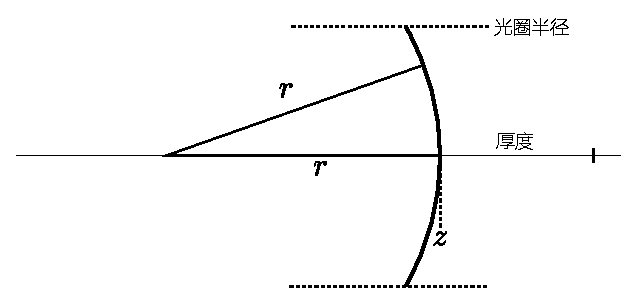
\includegraphics[width=0.6\linewidth]{chap06/Lenselement.eps}
    \caption{透镜界面(实曲线)与光轴相交于位置$z$。界面几何形状由
        表示其在光轴上下方范围的光圈半径以及元件的曲率半径$r$描述。
        如果元件有球形横截面,则它的轮廓由球心在光轴上距离$r$的球体给定,
        该球体也穿过$z$。如果$r$是负的,则元件界面就如从场景中看到那样是凹的
        (如图所示);否则就是\protect\keyindex{凸}{convex}{}的。透镜厚度给出了到
        右边下一个界面的距离,或者对于最右边的界面是到胶片平面的距离。}
    \label{fig:6.17}
\end{figure}

结构体\refvar{LensElementInterface}{}表示单个透镜元件界面。
\begin{lstlisting}
`\initcode{RealisticCamera Private Declarations}{=}`
struct `\initvar{LensElementInterface}{}` {
    `\refvar{Float}{}` `\initvar{curvatureRadius}{}`;
    `\refvar{Float}{}` `\initvar{thickness}{}`;
    `\refvar{Float}{}` `\initvar[LensElementInterface::eta]{eta}{}`;
    `\refvar{Float}{}` `\initvar{apertureRadius}{}`;
};
\end{lstlisting}

这里没有介绍的代码片\refcode{Load element data from lens description file}{}
\sidenote{译者注:我补充回来了。}读取透镜元件
并初始化数组\refvar[elementInterfaces]{RealisticCamera::elementInterfaces}{}。
见源代码中的注释了解该文件格式的细节,它并行化\reftab{6.1}中的结构,
并见pbrt发行版中的目录{\ttfamily scenes/lenses}了解大量透镜描述示例。

对从文件读取的值做了两个调整:第一,透镜系统传统上用毫米单位描述,
但pbrt假设场景单位用米。因此,除了折射率外的域都按1/1000缩小。
第二,元件直径被除以二;在下面的代码中半径是用起来更方便的量。
\begin{lstlisting}
`\refcode{RealisticCamera Private Data}{+=}\lastnext{RealisticCameraPrivateData}`
std::vector<`\refvar{LensElementInterface}{}`> `\initvar{elementInterfaces}{}`;
\end{lstlisting}

加载完透镜界面描述后,让一些关于透镜系统的值随时可得是很有用的。
\refvar{LensRearZ}{()}和\refvar{LensFrontZ}{()}分别返回
透镜系统尾部和头部元件的$z$深度\sidenote{译者注:靠近胶片的是尾部,远离胶片的是头部。}。
注意返回的$z$深度在相机空间中,而不是透镜空间中,所以为正值。
\begin{lstlisting}
`\initcode{RealisticCamera Private Methods}{=}\initnext{RealisticCameraPrivateMethods}`
`\refvar{Float}{}` `\initvar{LensRearZ}{}`() const {
    return `\refvar{elementInterfaces}{}`.back().`\refvar{thickness}{}`;
}
\end{lstlisting}

求头部元件$z$位置需要求所有元件厚度之和(见\reffig{6.18})。
任何位于系统性能敏感部分的代码都不需要该值,
所以在需要时重算它就行。如果该方法对性能有影响,
最好还是在\refvar{RealisticCamera}{}中缓存该值。
\begin{figure}[htbp]
    \centering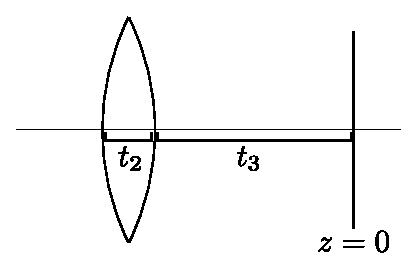
\includegraphics[width=0.4\linewidth]{chap06/Elementthicknessandposition.eps}
    \caption{元件厚度与光轴上位置的关系。胶片平面位于$z=0$,尾部元件的厚度$t_3$给出
        了从胶片到其界面的距离;这里尾部界面与轴交于$z=-t_3$。下一个元件厚度为$t_2$且
        位于$z=-t_3-t_2$,以此类推。头部元件交$z$轴于$\sum_i-t_i$。}
    \label{fig:6.18}
\end{figure}
\begin{lstlisting}
`\refcode{RealisticCamera Private Methods}{+=}\lastnext{RealisticCameraPrivateMethods}`
`\refvar{Float}{}` `\initvar{LensFrontZ}{}`() const {
    `\refvar{Float}{}` zSum = 0;
    for (const `\refvar{LensElementInterface}{}` &element : `\refvar{elementInterfaces}{}`)
        zSum += element.`\refvar{thickness}{}`;
    return zSum;
}
\end{lstlisting}

\refvar{RearElementRadius}{()}按单位米返回尾部元件光圈半径。
\begin{lstlisting}
`\refcode{RealisticCamera Private Methods}{+=}\lastnext{RealisticCameraPrivateMethods}`
`\refvar{Float}{}` `\initvar{RearElementRadius}{}`() const {
    return `\refvar{elementInterfaces}{}`.back().`\refvar{apertureRadius}{}`;
}
\end{lstlisting}
\subsection{追踪穿过透镜的光线}\label{sub:追踪穿过透镜的光线}
给定起始于透镜系统胶片一侧的光线,\refvar{TraceLensesFromFilm}{()}依次
计算与每个元件的相交处,如果其路径在穿过透镜系统途中被挡住了就终结该光线并返回{\ttfamily false}。
否则它就返回{\ttfamily true}并用相机空间中退出的光线来初始化{\ttfamily *rOut}。
在遍历时,{\ttfamily elementZ}追踪当前透镜元件的$z$截距。
因为光线起始于胶片,所以按照和\refvar{elementInterfaces}{}存储的相反顺序遍历透镜。
\begin{lstlisting}
`\refcode{RealisticCamera Method Definitions}{+=}\lastnext{RealisticCameraMethodDefinitions}`
bool `\refvar{RealisticCamera}{}`::`\initvar{TraceLensesFromFilm}{}`(const `\refvar{Ray}{}` &rCamera,
        `\refvar{Ray}{}` *rOut) const {
    `\refvar{Float}{}` elementZ = 0;
    `\refcode{Transform rCamera from camera to lens system space}{}`
    for (int i = `\refvar{elementInterfaces}{}`.size() - 1; i >= 0; --i) {
        const `\refvar{LensElementInterface}{}` &element = `\refvar{elementInterfaces}{}`[i];
        `\refcode{Update ray from film accounting for interaction with element}{}`
    }
    `\refcode{Transform rLens from lens system space back to camera space}{}`
    return true;
}
\end{lstlisting}

因为在pbrt的相机空间中相机指向$+z$轴但透镜在$-z$轴,
所以射线端点和方向的$z$分量需要取反。
尽管这是个简单到可以直接施加的变换,
我们还是偏好用显式的\refvar{Transform}{}使目的更明确。
\begin{lstlisting}
`\initcode{Transform rCamera from camera to lens system space}{=}`
static const `\refvar{Transform}{}` CameraToLens = `\refvar{Scale}{}`(1, 1, -1);
`\refvar{Ray}{}` rLens = CameraToLens(rCamera);
\end{lstlisting}

回想\reffig{6.18}中怎样计算元件的$z$截距:
因为我们从后往前访问元件,所以在考虑该元件的作用前
必须从{\ttfamily elementZ}中减去元件的厚度来计算其$z$截距。
\begin{lstlisting}
`\initcode{Update ray from film accounting for interaction with element}{=}`
elementZ -= element.`\refvar{thickness}{}`;
`\refcode{Compute intersection of ray with lens element}{}`
`\refcode{Test intersection point against element aperture}{}`
`\refcode{Update ray path for element interface interaction}{}`
\end{lstlisting}

有了元件的$z$轴截距,下一步是计算沿光线与元件界面(或光圈平面)相交处的参数值$t$。
对于光圈,采用光线-平面测试(见\refsub{光线-边界相交})。
对于球形界面,\refvar{IntersectSphericalElement}{()}执行该测试
并且如果找到相交处则还返回曲面法线;计算折射光方向时将需要该法线。
\begin{lstlisting}
`\initcode{Compute intersection of ray with lens element}{=}`
`\refvar{Float}{}` t;
`\refvar{Normal3f}{}` n;
bool isStop = (element.`\refvar{curvatureRadius}{}` == 0);
if (isStop)
    t = (elementZ - rLens.`\refvar[Ray::o]{o}{}`.z) / rLens.`\refvar[Ray::d]{d}{}`.z;
else {
    `\refvar{Float}{}` radius = element.`\refvar{curvatureRadius}{}`;
    `\refvar{Float}{}` zCenter = elementZ + element.`\refvar{curvatureRadius}{}`;
    if (!`\refvar{IntersectSphericalElement}{}`(radius, zCenter, rLens, &t, &n))
        return false;
}
\end{lstlisting}

方法\refvar{IntersectSphericalElement}{()}大致
和\refvar{Sphere::Intersect}{()}一样,不过它专门针对
元件中心在$z$轴上(且因此中心的$x$和$y$分量为零)这一情况。
这里文中没有包含代码片\refcode{Compute t0 and t1 for ray-element intersection}{}
和\refcode{Compute surface normal of element at ray intersection point}{},因为它们和
\refvar{Sphere::Intersect}{()}的实现一样\sidenote{译者注:我补充回来了。}。
\begin{lstlisting}
`\refcode{RealisticCamera Method Definitions}{+=}\lastnext{RealisticCameraMethodDefinitions}`
bool `\refvar{RealisticCamera}{}`::`\initvar{IntersectSphericalElement}{}`(`\refvar{Float}{}` radius,
        `\refvar{Float}{}` zCenter, const `\refvar{Ray}{}` &ray, `\refvar{Float}{}` *t, `\refvar{Normal3f}{}` *n) {
    `\refcode{Compute t0 and t1 for ray-element intersection}{}`
    `\refcode{Select intersection  based on ray direction and element curvature}{}`
    `\refcode{Compute surface normal of element at ray intersection point}{}`
    return true;
}
\end{lstlisting}
\begin{lstlisting}
`\initcode{Compute t0 and t1 for ray-element intersection}{=}`
`\refvar{Point3f}{}` o = ray.`\refvar[Ray::o]{o}{}` - `\refvar{Vector3f}{}`(0, 0, zCenter);
`\refvar{Float}{}` A = ray.`\refvar[Ray::d]{d}{}`.x*ray.`\refvar[Ray::d]{d}{}`.x + ray.`\refvar[Ray::d]{d}{}`.y*ray.`\refvar[Ray::d]{d}{}`.y + ray.`\refvar[Ray::d]{d}{}`.z*ray.`\refvar[Ray::d]{d}{}`.z;
`\refvar{Float}{}` B = 2 * (ray.`\refvar[Ray::d]{d}{}`.x*o.x + ray.`\refvar[Ray::d]{d}{}`.y*o.y + ray.`\refvar[Ray::d]{d}{}`.z*o.z);
`\refvar{Float}{}` C = o.x*o.x + o.y*o.y + o.z*o.z - radius*radius;
`\refvar{Float}{}` t0, t1;
if (!`\refvar{Quadratic}{}`(A, B, C, &t0, &t1))
    return false;
\end{lstlisting}
\begin{lstlisting}
`\initcode{Compute surface normal of element at ray intersection point}{=}`
*n = `\refvar{Normal3f}{}`(`\refvar{Vector3f}{}`(o + *t * ray.`\refvar[Ray::d]{d}{}`));
*n = `\refvar{Faceforward}{}`(`\refvar{Normalize}{}`(*n), -ray.`\refvar[Ray::d]{d}{}`);
\end{lstlisting}

然而这里在选择返回哪个交点时有个微妙之处\sidenote{译者注:原文subtlety。}:
$t>0$的最近相交处不一定在元件界面上;
见\reffig{6.19}\footnote{“微妙之处”(subtlety)一般意味着作者花费好几个小时来调试它。}。
例如,对于自场景中接近并与(具有负曲率半径的)凹透镜相交的光线,
两个相交处中不管近处那个是否有$t>0$都该返回远处那个。
幸运的是,基于光线方向和曲率半径的简单逻辑可指明用哪个$t$值。
\begin{figure}[htbp]
    \centering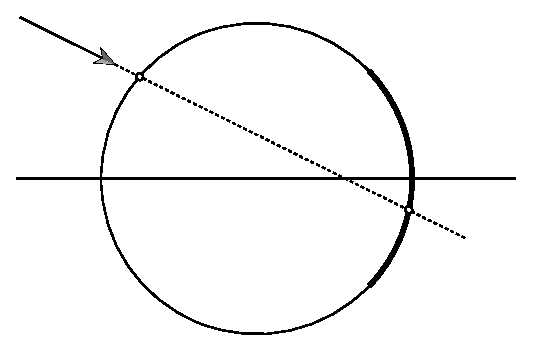
\includegraphics[width=0.5\linewidth]{chap06/Lenscorrectintersection.eps}
    \caption{当计算光线与球形透镜元件的相交处时,光线与整球的首个相交处不一定是我们想要的。
        这里,第二个相交处才在真正的元件界面(粗线)上,而第一个应该被忽略。}
    \label{fig:6.19}
\end{figure}
\begin{lstlisting}
`\initcode{Select intersection  based on ray direction and element curvature}{=}`
bool useCloserT = (ray.`\refvar[Ray::d]{d}{}`.z > 0) ^ (radius < 0);
*t = useCloserT ? std::min(t0, t1) : std::max(t0, t1);
if (*t < 0)
    return false;
\end{lstlisting}

每个透镜元件都按某半径绕光轴扩展;如果与该元件的交点在该半径之外,
则该光线实际上将与镜头罩相交并终止。
类似地,如果光线与光圈相交,它也会终止。
因此,这里我们用当前元件的适用限制来测试交点,
要么终止该光线,要么它幸存下来并将其端点更新为当前交点。
\begin{lstlisting}
`\initcode{Test intersection point against element aperture}{=}`
`\refvar{Point3f}{}` pHit = rLens(t);
`\refvar{Float}{}` r2 = pHit.x * pHit.x + pHit.y * pHit.y;
if (r2 > element.`\refvar{apertureRadius}{}` * element.`\refvar{apertureRadius}{}`)
    return false;
rLens.`\refvar[Ray::o]{o}{}` = pHit;
\end{lstlisting}

如果当前元件是光圈,则光路在穿过元件界面时不受影响。
对于玻璃(或塑料)透镜元件,光线在从具有某个折射率的介质进入
到具有另一折射率的介质时在交界面会改变方向
(光线可能从空气进入玻璃、从玻璃进入空气,或者从
具有某个折射率的玻璃进入具有不同折射率的另一种玻璃)。

\refsec{镜面反射与透射}讨论了两种介质边界间折射率的变化
将怎样改变光线的方向及其携带的辐射量(这里的情况下
我们可以忽略辐射量的变化,因为如果光线在进入和退出透镜系统时
处于同一种介质中则这种效应会抵消掉——这里都是空气)。
函数\refvar{Refract}{()}定义在\refsub{镜面透射};
注意它预设入射方向指向远离曲面的方向,所以传入前要对光线方向取反。
该函数在出现\keyindex{全内反射}{total internal reflection}{reflection反射}时
返回{\ttfamily false},该情况下光路终止。
否则在{\ttfamily w}中返回折射方向。

通常,穿过这类界面时一些光被透射而另一些被反射。
这里我们忽略反射并假设完美传输。尽管这是种近似,但它是合理的:
制造透镜时一般用了设计的涂料把反射降低到光线所带辐射的0.25\%左右
(然而,对这少量的反射建模对于实现\keyindex{镜头光晕}{lens flare}{}会很重要)。
\begin{lstlisting}
`\initcode{Update ray path for element interface interaction}{=}`
if (!isStop) {
    `\refvar{Vector3f}{}` w;
    `\refvar{Float}{}` etaI = element.`\refvar[LensElementInterface::eta]{eta}{}`;
    `\refvar{Float}{}` etaT = (i > 0 && `\refvar{elementInterfaces}{}`[i - 1].`\refvar[LensElementInterface::eta]{eta}{}` != 0) ?
        `\refvar{elementInterfaces}{}`[i - 1].`\refvar[LensElementInterface::eta]{eta}{}` : 1;
    if (!`\refvar{Refract}{}`(`\refvar{Normalize}{}`(-rLens.`\refvar[Ray::d]{d}{}`), n, etaI / etaT, &w))
        return false;
    rLens.`\refvar[Ray::d]{d}{}` = w;
}
\end{lstlisting}

若光线成功从前端透镜元件射出,它只需要从透镜空间变换到相机空间。
\begin{lstlisting}
`\initcode{Transform rLens from lens system space back to camera space}{=}`
if (rOut != nullptr) {
    static const `\refvar{Transform}{}` LensToCamera = `\refvar{Scale}{}`(1, 1, -1);
    *rOut = LensToCamera(rLens);
}
\end{lstlisting}

方法\refvar{TraceLensesFromScene}{()}和\refvar{TraceLensesFromFilm}{()}非常相似,这里不再介绍。
主要差别在于它是从前往后而不是从后往前遍历元件。
注意它假设传入的光线已经在相机空间了;
如果光线始于世界空间则调用者应负责执行该变换。
返回的光线位于尾部透镜元件朝向胶片的相机空间中。
\begin{lstlisting}
`\refcode{RealisticCamera Private Methods}{+=}\lastcode{RealisticCameraPrivateMethods}`
bool `\initvar{TraceLensesFromScene}{}`(const `\refvar{Ray}{}` &rCamera, `\refvar{Ray}{}` *rOut) const;
\end{lstlisting}

\subsection{厚透镜近似}\label{sub:厚透镜近似}
\refsub{薄透镜模型与景深}中用的薄透镜近似是基于透镜系统沿光轴厚度为0的简化假设。
透镜系统的厚透镜近似因为考虑了透镜系统的$z$范围而更精确些。
这里在介绍厚透镜的基本概念之后,我们将用厚透镜近似来确定
要把透镜系统放在离胶片多远处来对焦\refsub{对焦}中想要的对焦深度。

厚透镜近似将透镜系统表示为两对沿光轴的距离——
\keyindex{焦点}{focal point}{}以及\keyindex{主平面}{principal plane}{};
一个透镜系统有两个\keyindex{主点}{cardinal point}{}。
如果经由一个理想透镜系统追踪平行于光轴的光线,
则所有这些光线将会交于光轴上同一点——这就是焦点
(实际中,真实透镜系统并不绝对理想,不同高度的入射光线
与光轴将相交于一个$z$值小范围——这就是\keyindex{球面像差}{spherical aberration}{aberration像差})。
有了特定的透镜系统,我们就能从每一侧追踪穿过它且与光轴平行的光线,
并计算它们与$z$轴的相交处以找到焦点(见\reffig{6.20})。
\begin{figure}[htbp]
    \centering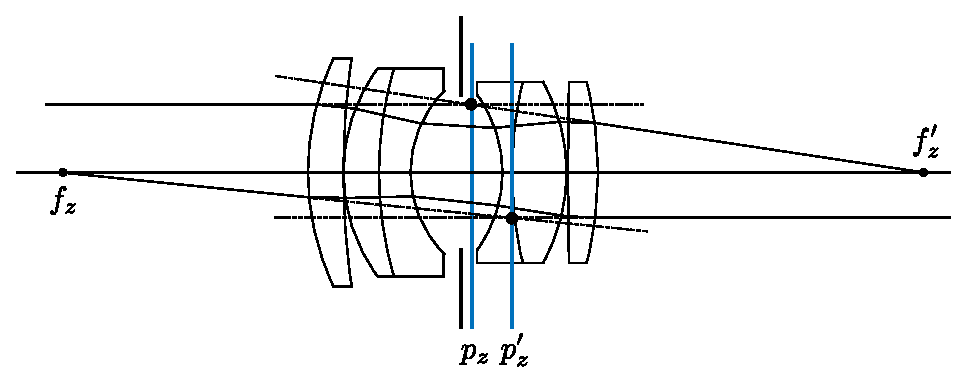
\includegraphics[width=\linewidth]{chap06/Lenssystemcardinalpoints.eps}
    \caption{计算透镜系统的主点。文件{\ttfamily lenses/dgauss.dat}中
    描述的透镜系统,来自场景的入射光线平行于光轴(轴上方),
    来自胶片的光线平行于光轴(下方)。这些入射光线对应的
    离开透镜系统的光线与光轴的相交处给出了两个焦点$f'_z$(胶片一侧)
    和$f_z$(场景一侧)。每对入射和出射光线的延长线以及原始光线的相交处给定了
    主平面$z=p_z$和$z=p'_z$,这里表示为垂直于光轴的蓝线。}
    \label{fig:6.20}
\end{figure}

每个主平面通过延长平行于光轴的入射光线以及离开透镜的光线直至相交来求得;
相交处的$z$深度给出了对应主平面的深度。\reffig{6.20}展示了
一个透镜系统及其焦点$f_z$和$f'_z$以及位于$z$值$p_z$和$p'_z$的主平面
(正如\refsub{薄透镜模型与景深},有撇的变量表示透镜系统胶片一侧的点,
无撇的变量表示场景中要成像的点)。

给定离开透镜的光线,求焦点要先计算光线的$x$和$y$分量为零时的值$t_{\mathrm{f}}$。
若进入的光线只沿$x$偏移了光轴,则我们要求出
使$o_x+t_{\mathrm{f}}d_x=0$的$t_{\mathrm{f}}$。因此
\begin{align*}
    t_{\mathrm{f}}=\frac{-o_x}{d_x}\, .
\end{align*}
同样的方法,为了求得离开透镜的光线与原始光线有相同高度处
的主平面的$t_{\mathrm{p}}$,我们有$o_x+t_{\mathrm{p}}d_x=x$,因此
\begin{align*}
    t_{\mathrm{p}}=\frac{x-o_x}{d_x}\, .
\end{align*}
一旦算出这两个$t$值,射线方程就可用于求得对应点的$z$坐标。

方法\refvar{ComputeCardinalPoints}{()}为给定光线计算焦点和主平面的$z$深度。
注意它假设光线在相机空间中但返回透镜空间中沿光轴的$z$值。
\begin{lstlisting}
`\refcode{RealisticCamera Method Definitions}{+=}\lastnext{RealisticCameraMethodDefinitions}`
void `\refvar{RealisticCamera}{}`::`\initvar{ComputeCardinalPoints}{}`(const `\refvar{Ray}{}` &rIn,
        const `\refvar{Ray}{}` &rOut, `\refvar{Float}{}` *pz, `\refvar{Float}{}` *fz) {
    `\refvar{Float}{}` tf = -rOut.`\refvar[Ray::o]{o}{}`.x / rOut.`\refvar[Ray::d]{d}{}`.x;
    *fz = -rOut(tf).z;
    `\refvar{Float}{}` tp = (rIn.`\refvar[Ray::o]{o}{}`.x - rOut.`\refvar[Ray::o]{o}{}`.x) / rOut.`\refvar[Ray::d]{d}{}`.x;
    *pz = -rOut(tp).z;
}
\end{lstlisting}

方法\refvar{ComputeThickLensApproximation}{()}为透镜系统
计算两对主点。
\begin{lstlisting}
`\refcode{RealisticCamera Method Definitions}{+=}\lastnext{RealisticCameraMethodDefinitions}`
void `\refvar{RealisticCamera}{}`::`\initvar{ComputeThickLensApproximation}{}`(`\refvar{Float}{}` pz[2],
        `\refvar{Float}{}` fz[2]) const {
    `\refcode{Find height x from optical axis for parallel rays}{}`
    `\refcode{Compute cardinal points for film side of lens system}{}`
    `\refcode{Compute cardinal points for scene side of lens system}{}`
}
\end{lstlisting}

首先,我们必须为追踪的光线选择沿$x$轴的高度。
它应该离$x=0$足够远使得有足够数值精度来准确计算
离开透镜系统的光线与$z$轴相交于哪里,
但$x$轴上也不能太高以免在光线穿过透镜系统时命中光圈。
这里,我们采用胶片对角范围的很小比例;其效果一般很好,除非光圈非常小。
\begin{lstlisting}
`\initcode{Find height x from optical axis for parallel rays}{=}`
`\refvar{Float}{}` x = .001 * `\refvar{film}{}`->`\refvar{diagonal}{}`;
\end{lstlisting}

为了构建从场景进入透镜系统的光线{\ttfamily rScene},
我们从透镜前端偏移一点(回想传入\refvar{TraceLensesFromScene}{()}的
光线应该在相机空间)。
\begin{lstlisting}
`\initcode{Compute cardinal points for film side of lens system}{=}`
`\refvar{Ray}{}` rScene(`\refvar{Point3f}{}`(x, 0, `\refvar{LensFrontZ}{}`() + 1), `\refvar{Vector3f}{}`(0, 0, -1));
`\refvar{Ray}{}` rFilm;
`\refvar{TraceLensesFromScene}{}`(rScene, &rFilm);
`\refvar{ComputeCardinalPoints}{}`(rScene, rFilm, &pz[0], &fz[0]);
\end{lstlisting}

从透镜系统胶片一侧起始的等价过程为我们给出了另外两个主点。
\begin{lstlisting}
`\initcode{Compute cardinal points for scene side of lens system}{=}`
rFilm = `\refvar{Ray}{}`(`\refvar{Point3f}{}`(x, 0, `\refvar{LensRearZ}{}`() - 1), `\refvar{Vector3f}{}`(0, 0, 1));
`\refvar{TraceLensesFromFilm}{}`(rFilm, &rScene);
`\refvar{ComputeCardinalPoints}{}`(rFilm, rScene, &pz[1], &fz[1]);
\end{lstlisting}

\subsection{对焦}\label{sub:对焦}
透镜系统可以通过相对于胶片移动来对焦场景中的指定深度,
这样在想要的对焦深度处的点成像为胶片平面上的一点。
高斯透镜方程\refeq{6.3}给了我们一个可解的关系来对焦厚透镜。

对于厚透镜,高斯透镜方程把到场景中位于$z$处的点的距离
和它对焦到$z'$的点用下式联系起来:
\begin{align}\label{eq:6.3}
    \frac{1}{z'-p'_z}-\frac{1}{z-p_z}=\frac{1}{f}\, .
\end{align}
对于薄透镜,$p_z=p'_z=0$,即推出\refeq{6.1}。

如果我们知道主平面的位置$p_z$和$p'_z$以及透镜的焦距$f$
并想要对焦沿光轴的某个深度$z$,则我们需确定应将系统平移多远$\delta$使得
\begin{align*}
    \frac{1}{z'-p'_z+\delta}-\frac{1}{z-p_z+\delta}=\frac{1}{f}\, .
\end{align*}

胶片一侧的焦点应在胶片上,所以$z'=0$,且$z=z_{\mathrm{f}}$即给定的对焦深度。
唯一未知的是$\delta$,一些代数处理为我们给出
\begin{align}\label{eq:6.4}
    \delta=\frac{1}{2}\left(p_z-z_{\mathrm{f}}+p'_z-\sqrt{(p_z-z_{\mathrm{f}}-p'_z)(p_z-z_{\mathrm{f}}-4f-p'_z)}\right)\, .
\end{align}
(实际上有两个解,但两个中更近的这个解给出了对透镜位置较小的调整,因此是合适的那个。)

\refvar{FocusThickLens}{()}用该近似对焦透镜系统。
计算$\delta$后,它返回应放置透镜系统处沿$z$轴离胶片的偏移量。
\begin{lstlisting}
`\refcode{RealisticCamera Method Definitions}{+=}\lastnext{RealisticCameraMethodDefinitions}`
`\refvar{Float}{}` `\refvar{RealisticCamera}{}`::`\initvar{FocusThickLens}{}`(`\refvar{Float}{}` focusDistance) {
    `\refvar{Float}{}` pz[2], fz[2];
    `\refvar{ComputeThickLensApproximation}{}`(pz, fz);
    `\refcode{Compute translation of lens, delta, to focus at focusDistance}{}`
    return `\refvar{elementInterfaces}{}`.back().`\refvar{thickness}{}` + delta;
}
\end{lstlisting}

\refeq{6.4}给出了偏移量$\delta$。透镜的焦距$f$是主点$f'_z$和$p'_z$间的距离。
还要注意对于$z$用的是对焦距离
\sidenote{译者注:和\refsec{投影相机模型}中的“focal distance”不同,这里的原文是“focus distance”。}
的相反数,因为光轴指向负的$z$。
\begin{lstlisting}
`\initcode{Compute translation of lens, delta, to focus at focusDistance}{=}`
`\refvar{Float}{}` f = fz[0] - pz[0];
`\refvar{Float}{}` z = -focusDistance;
`\refvar{Float}{}` delta = 0.5f * (pz[1] - z + pz[0] -
    std::sqrt((pz[1] - z - pz[0]) * (pz[1] - z - 4 * f - pz[0])));
\end{lstlisting}

我们现在终于可以实现\refvar{RealisticCamera}{}构造函数中
对焦透镜系统的代码片了(回想最尾部元件界面的厚度是该界面到胶片的距离)。
\begin{lstlisting}
`\initcode{Compute lens-film distance for given focus distance}{=}`
`\refvar{elementInterfaces}{}`.back().`\refvar{thickness}{}` = `\refvar{FocusThickLens}{}`(focusDistance);
\end{lstlisting}

\subsection{出射瞳}\label{sub:出射瞳}
不是所有从胶片平面上给定点起始朝向尾部透镜元件的光线都能成功射出透镜系统;
一些会被光圈阻挡或者与透镜系统外壳相交。
反过来,尾部透镜元件上不是所有点都能把辐射传输到胶片上的点。
尾部元件上确实能带着光通过透镜系统的点集称为\keyindex{出射瞳}{exit pupil}{pupil瞳};
它的尺寸和位置随着胶片平面上的视点变化
(类似地,\keyindex{入射瞳}{entrance pupil}{pupil瞳}是场景中给定点起始
且能到达胶片的光线所穿过的前端透镜元件区域)
\sidenote{译者注:这和后文补充材料\refsub{光圈}中对出射瞳与入射瞳的定义有一些出入,请读者酌情采信。}。

\reffig{6.21}展示了广角镜头从胶片平面上两点看到的出射瞳。
当点靠近胶片边缘时出射瞳更小。这类收缩的一个结果是暗角。
\begin{figure}[htbp]
    \centering
    \subfloat[]{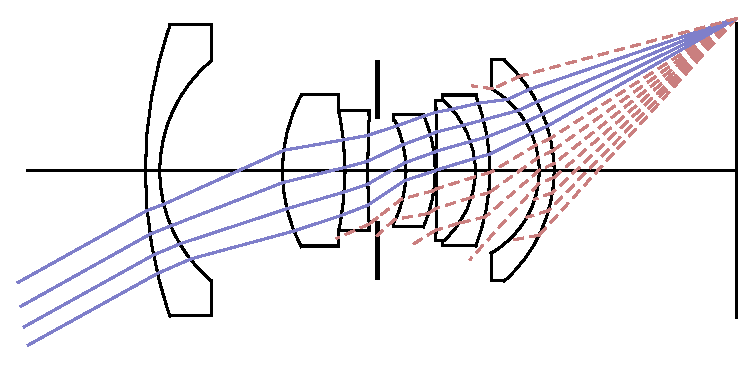
\includegraphics[width=0.5\linewidth]{chap06/wide22-rays-edge.eps}\label{fig:6.21.1}}\qquad
    \subfloat[]{
\includegraphics[width=0.2\linewidth]{chap06/wide22-exit-edge.eps}\label{fig:6.21.2}}\\
    \subfloat[]{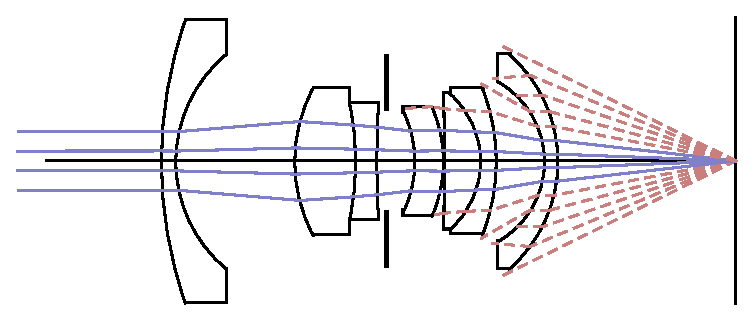
\includegraphics[width=0.5\linewidth]{chap06/wide22-rays-middle.eps}\label{fig:6.21.3}}\qquad
    \subfloat[]{
\includegraphics[width=0.2\linewidth]{chap06/wide22-exit-middle.eps}\label{fig:6.21.4}}
    \caption{22mm广角镜头在5.5mm光圈(f/4)下的出射瞳。
        (a)起始于胶片平面边缘一点的光线进入尾部透镜元件的多个点。
        虚线表示被阻挡而没有射出透镜系统的光线。
        (b)从(a)中的有利位置看到的出射瞳的像。尾部透镜元件是黑色的,而出射瞳表示为灰色。
        (c)在胶片中心,不同的出射瞳区域允许光线射出到场景中。
        (d)从胶片中心看到的出射瞳的像。}
    \label{fig:6.21}
\end{figure}

当追踪起始于胶片的光线时,我们想避免追踪太多没能穿过透镜系统的光线;
因此值得把采样限制在出射瞳本身及其周围很小区域内,
而不是浪费地在尾部透镜元件整个区域上采样。

在追踪光线前计算胶片上每点的出射瞳会开销极大;相反\refvar{RealisticCamera}{}
的实现预先计算沿胶片平面上的直线段对应的出射瞳边界。
因为我们假设透镜系统是绕光轴径向对称的,所以出射瞳边界也会是径向对称的,
且胶片平面上任意点的边界都可以通过适当旋转这些线段边界来求得(\reffig{6.22})
\sidenote{译者注:\protect\reffig{6.22}题注最后一句翻译不确定是否正确。}。
然后这些边界用于为特定胶片采样位置高效求取出射瞳边界。
\begin{figure}[htbp]
    \centering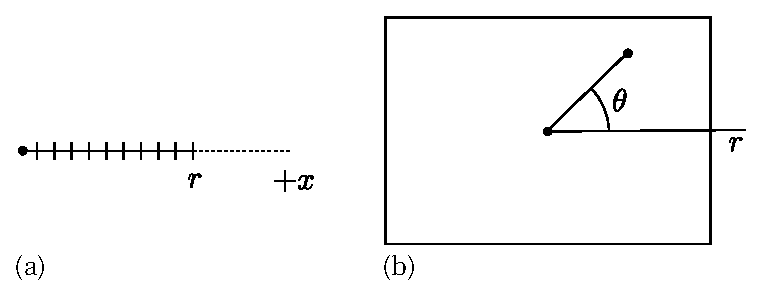
\includegraphics[width=0.7\linewidth]{chap06/Exitpupilboundsfilm.eps}
    \caption{预先计算出射瞳边界。(a)\refvar{RealisticCamera}{}为胶片平面上
        沿$x$轴的一系列线段计算出射瞳的边界,直到达到胶片中心到角点的距离$r$。
        (b)鉴于径向对称的假设,我们可以通过计算点与$x$轴间的夹角$\theta$来
        为胶片上的任意点(实心点)求取出射瞳边界。如果初始出射瞳边界内的一点被采样
        再旋转$\theta$,则我们就有了原始点处出射瞳内的一点。}
    \label{fig:6.22}
\end{figure}

需要意识到的一个重要细节是,由于透镜系统通过沿光轴平移来对焦,
所以当调整透镜系统的对焦时出射瞳的形状和位置会变化。
因此在对焦后才计算这些边界十分重要
\footnote{作者也是调试几个小时后才痛苦地吸取这一教训。}。
\begin{lstlisting}
`\initcode{Compute exit pupil bounds at sampled points on the film}{=}`
int nSamples = 64;
`\refvar{exitPupilBounds}{}`.resize(nSamples);
`\refvar{ParallelFor}{}`(
    [&](int i) {
        `\refvar{Float}{}` r0 = (`\refvar{Float}{}`)i / nSamples * `\refvar{film}{}`->`\refvar{diagonal}{}` / 2;
        `\refvar{Float}{}` r1 = (`\refvar{Float}{}`)(i + 1) / nSamples * `\refvar{film}{}`->`\refvar{diagonal}{}` / 2;
        `\refvar{exitPupilBounds}{}`[i] = `\refvar{BoundExitPupil}{}`(r0, r1);
    }, nSamples);
\end{lstlisting}
\begin{lstlisting}
`\refcode{RealisticCamera Private Data}{+=}\lastcode{RealisticCameraPrivateData}`
std::vector<`\refvar{Bounds2f}{}`> `\initvar{exitPupilBounds}{}`;
\end{lstlisting}

方法\refvar{BoundExitPupil}{()}计算从胶片平面上一段点所见出射瞳的2D边界框。
通过尝试追踪在尾部透镜元件切平面的一组点上穿过透镜系统的光线来求取该边界框。
成功穿过透镜系统的光线的边界框便给出了出射瞳的大致边界——见\reffig{6.23}
\sidenote{译者注:\reffig{6.23}题注最后两句的意思是:尾部透镜元件在其切平面
    上的投影范围作为光线方向向量(归一化前)终点的采样范围,胶片上的区间作为光线起点的采样范围;
    采样许多这样的光线,保留其中成功穿过透镜系统的光线,这些光线穿过尾部透镜切平面时
    的位置即大致给出了出射瞳范围。}。
\begin{figure}[htbp]
    \centering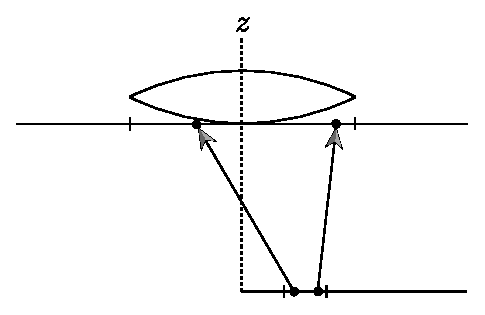
\includegraphics[width=0.5\linewidth]{chap06/Sampleexitpupil.eps}
    \caption{怎样计算出射瞳边界的2D图示。\refvar{BoundExitPupil}{()}接收
        胶片上沿$x$轴的区间。它沿区间采样一系列点(图的下方)。
        对于每个点,它还采样尾部透镜元件在与其尾部相切的平面上相应范围边框内的一点。
        它计算所有起始于区间的点且成功穿过透镜系统的光线在切平面上的边界框。}
    \label{fig:6.23}
\end{figure}
\begin{lstlisting}
`\refcode{RealisticCamera Method Definitions}{+=}\lastnext{RealisticCameraMethodDefinitions}`
`\refvar{Bounds2f}{}` `\refvar{RealisticCamera}{}`::`\initvar{BoundExitPupil}{}`(`\refvar{Float}{}` pFilmX0,
        `\refvar{Float}{}` pFilmX1) const {
    `\refvar{Bounds2f}{}` pupilBounds;
    `\refcode{Sample a collection of points on the rear lens to find exit pupil}{}`
    `\refcode{Return entire element bounds if no rays made it through the lens system}{}`
    `\refcode{Expand bounds to account for sample spacing}{}`
    return pupilBounds;
}
\end{lstlisting}

该实现非常密集地采样出射瞳——每段共有$1024^2$个点。
我们发现实践中该采样率能提供很好的出射瞳边界。
\begin{lstlisting}
`\initcode{Sample a collection of points on the rear lens to find exit pupil}{=}`
const int nSamples = 1024 * 1024;
int nExitingRays = 0;
`\refcode{Compute bounding box of projection of rear element on sampling plane}{}`
for (int i = 0; i < nSamples; ++i) {
    `\refcode{Find location of sample points on x segment and rear lens element}{}`
    `\refcode{Expand pupil bounds if ray makes it through the lens system}{}`
}
\end{lstlisting}

尾部元件在与之相切\sidenote{译者注:原文误写为垂直,已修正。}的平面上
的边界框不足以成为出射瞳在该平面上的投影的保守边界框;
因为元件一般是曲形的,穿过该平面边界之外的光线可能自己与尾部透镜元件有效范围相交。
比起计算精确边界,我们则是大幅增大边框。结果是用来计算出射瞳边界而采样的许多点会被浪费;
实践中,这是很小的代价,因为通常这些样本在透镜的光线追踪阶段会很快被终止。
\begin{lstlisting}
`\initcode{Compute bounding box of projection of rear element on sampling plane}{=}`
`\refvar{Float}{}` rearRadius = `\refvar{RearElementRadius}{}`();
`\refvar{Bounds2f}{}` projRearBounds(`\refvar{Point2f}{}`(-1.5f * rearRadius, -1.5f * rearRadius),
                        `\refvar{Point2f}{}`( 1.5f * rearRadius,  1.5f * rearRadius));
\end{lstlisting}

通过在$x$区间端点间线性插值来求得胶片上的$x$样本点。
稍后\refsub{Hammersley和Halton序列}{}定义的函数\refvar{RadicalInverse}{()}用于
为出射瞳边界框内的采样点计算插值偏移量。我们将看到
这里实现的采样策略对应于在3D中使用Hammersley点;
得到的点集会最小化整个3D域覆盖情况的差异,反过来保证了准确估计出射瞳边界。
\begin{lstlisting}
`\initcode{Find location of sample points on x segment and rear lens element}{=}`
`\refvar{Point3f}{}` pFilm(`\refvar{Lerp}{}`((i + 0.5f) / nSamples, pFilmX0, pFilmX1), 0, 0);
`\refvar{Float}{}` u[2] = { `\refvar{RadicalInverse}{}`(0, i), `\refvar{RadicalInverse}{}`(1, i) };
`\refvar{Point3f}{}` pRear(`\refvar{Lerp}{}`(u[0], projRearBounds.pMin.x, projRearBounds.pMax.x),
              `\refvar{Lerp}{}`(u[1], projRearBounds.pMin.y, projRearBounds.pMax.y),
              `\refvar{LensRearZ}{}`());
\end{lstlisting}

现在我们可构造从{\ttfamily pFilm}到{\ttfamily pRear}的光线并
通过看它是否成功射出透镜系统前端来确定它是否在出射瞳内。
如果是,则拓展出射瞳边界以包含该点。如果采样点已经在
目前算出的出射瞳边界框内,则我们可以跳过光线追踪步骤以节约些无用功。
\begin{lstlisting}
`\initcode{Expand pupil bounds if ray makes it through the lens system}{=}`
if (`\refvar{Inside}{}`(`\refvar{Point2f}{}`(pRear.x, pRear.y), pupilBounds) ||
    `\refvar{TraceLensesFromFilm}{}`(`\refvar{Ray}{}`(pFilm, pRear - pFilm), nullptr)) {
    pupilBounds = `\refvar[Union1]{Union}{}`(pupilBounds, `\refvar{Point2f}{}`(pRear.x, pRear.y));
    ++nExitingRays;
}
\end{lstlisting}

可能没有样本光线能成功穿过透镜系统;例如一些在胶片范围边缘处出射瞳会消失的
超大广角镜头完全可能发生这种情况。这种情况下边界并不重要,
\refvar{BoundExitPupil}{()}返回包括了整个尾部透镜元件的边界。
\begin{lstlisting}
`\initcode{Return entire element bounds if no rays made it through the lens system}{=}`
if (nExitingRays == 0) 
    return projRearBounds;
\end{lstlisting}

当一个样本成功穿过透镜系统而它的一个相邻样本没有时,
有可能与该邻居很相近的另一个样本实际上能成功穿过。
因此,最终边界在每个方向上再大致按样本间距拓展以考虑这一不确定性。
\begin{lstlisting}
`\initcode{Expand bounds to account for sample spacing}{=}`
pupilBounds = `\refvar{Expand}{}`(pupilBounds,
                     2 * projRearBounds.`\refvar{Diagonal}{}`().`\refvar{Length}{}`() /
                     std::sqrt(nSamples));
\end{lstlisting}

有了预先计算并存储在\refvar[exitPupilBounds]{RealisticCamera::exitPupilBounds}{}中的边界,
方法\refvar{SampleExitPupil}{()}就能很高效地为胶片平面上的给定点求得出射瞳边界。
为了准确地对成像辐射度量学建模,下列代码需要知道该边界框的面积,
所以它通过{\ttfamily sampleBoundsArea}返回。
\begin{lstlisting}
`\refcode{RealisticCamera Method Definitions}{+=}\lastnext{RealisticCameraMethodDefinitions}` 
`\refvar{Point3f}{}` `\refvar{RealisticCamera}{}`::`\initvar{SampleExitPupil}{}`(const `\refvar{Point2f}{}` &pFilm,
        const `\refvar{Point2f}{}` &lensSample, `\refvar{Float}{}` *sampleBoundsArea) const {
    `\refcode{Find exit pupil bound for sample distance from film center}{}`
    `\refcode{Generate sample point inside exit pupil bound}{}`
    `\refcode{Return sample point rotated by angle of pFilm with +x axis}{}`
}
\end{lstlisting}
\begin{lstlisting}
`\initcode{Find exit pupil bound for sample distance from film center}{=}`
`\refvar{Float}{}` rFilm = std::sqrt(pFilm.x * pFilm.x + pFilm.y * pFilm.y);
int rIndex = rFilm / (`\refvar{film}{}`->`\refvar{diagonal}{}` / 2) * `\refvar{exitPupilBounds}{}`.size();
rIndex = std::min((int)`\refvar{exitPupilBounds}{}`.size() - 1, rIndex);
`\refvar{Bounds2f}{}` pupilBounds = `\refvar{exitPupilBounds}{}`[rIndex];
if (sampleBoundsArea) *sampleBoundsArea = pupilBounds.Area();
\end{lstlisting}

给定瞳的边界框后,通过对提供的位于$[0,1)^2$的值{\ttfamily lensSample}线性插值
来采样边界框中的一点。
\begin{lstlisting}
`\initcode{Generate sample point inside exit pupil bound}{=}`
`\refvar{Point2f}{}` pLens = pupilBounds.`\refvar[Bounds3::Lerp]{Lerp}{}`(lensSample);
\end{lstlisting}

因为出射瞳边界是从胶片上一点沿$+x$轴算得的,
但点{\ttfamily pFilm}是胶片上的任意点,
故出射瞳边框内的样本点必须像{\ttfamily pFilm}对$+x$轴那样旋转相同角度。
\begin{lstlisting}
`\initcode{Return sample point rotated by angle of pFilm with +x axis}{=}`
`\refvar{Float}{}` sinTheta = (rFilm != 0) ? pFilm.y / rFilm : 0;
`\refvar{Float}{}` cosTheta = (rFilm != 0) ? pFilm.x / rFilm : 1;
return `\refvar{Point3f}{}`(cosTheta * pLens.x - sinTheta * pLens.y,
               sinTheta * pLens.x + cosTheta * pLens.y,
               `\refvar{LensRearZ}{}`());
\end{lstlisting}

\subsection{生成光线}\label{sub:生成光线}
现在我们有了机制去追踪穿过透镜系统的光线并采样由胶片平面上的点得来的出射瞳边界内的点,
将\refvar{CameraSample}{}转化为离开相机的光线非常简单:
我们需要计算样本在胶片平面上的位置并生成起始于该点射向尾部透镜元件的光线,
然后通过透镜系统追踪它。
\begin{lstlisting}
`\refcode{RealisticCamera Method Definitions}{+=}\lastcode{RealisticCameraMethodDefinitions}`
`\refvar{Float}{}` `\refvar{RealisticCamera}{}`::`\initvar[RealisticCamera::GenerateRay]{\refvar{GenerateRay}{}}{}`(const `\refvar{CameraSample}{}` &sample,
        `\refvar{Ray}{}` *ray) const {
    `\refcode{Find point on film, pFilm, corresponding to sample.pFilm}{}`
    `\refcode{Trace ray from pFilm through lens system}{}`
    `\refcode{Finish initialization of RealisticCamera ray}{}`
    `\refcode{Return weighting for RealisticCamera ray}{}`
}
\end{lstlisting}

值\refvar[pFilm]{CameraSample::pFilm}{}与图像的整个像素分辨率有关。
这里我们用传感器的物理模型来操作,所以我们开始先将样本转化回$[0,1)^2$中。
接着,通过用该样本值在其区域上线性插值来求得胶片上的对应点
\sidenote{译者注:我暂未理解为何下面第5行代码中$x$值会取相反数,欢迎读者提供帮助。
    详见\url{https://github.com/mmp/pbrt-v4/issues/233}
    和\url{https://github.com/mmp/pbrt-v3/issues/289}。}。
\begin{lstlisting}
`\initcode{Find point on film, pFilm, corresponding to sample.pFilm}{=}`
`\refvar{Point2f}{}` s(sample.`\refvar{pFilm}{}`.x / `\refvar{film}{}`->`\refvar{fullResolution}{}`.x,
          sample.`\refvar{pFilm}{}`.y / `\refvar{film}{}`->`\refvar{fullResolution}{}`.y);
`\refvar{Point2f}{}` pFilm2 = `\refvar{film}{}`->`\refvar{GetPhysicalExtent}{}`().`\refvar[Bounds3::Lerp]{Lerp}{}`(s);
`\refvar{Point3f}{}` pFilm(-pFilm2.x, pFilm2.y, 0);
\end{lstlisting}

然后\refvar{SampleExitPupil}{()}给我们尾部透镜元件切平面上的一点,
让我们确定了光线的方向。我们可追踪该光线穿过透镜系统。
若光线被光圈阻挡或没能成功穿过透镜系统,\refvar[RealisticCamera::GenerateRay]{GenerateRay}{()}返回权重0
(调用者应保证检查该情况)。
\begin{lstlisting}
`\initcode{Trace ray from pFilm through lens system}{=}`
`\refvar{Float}{}` exitPupilBoundsArea;
`\refvar{Point3f}{}` pRear = `\refvar{SampleExitPupil}{}`(`\refvar{Point2f}{}`(pFilm.x, pFilm.y), sample.`\refvar{pLens}{}`,
                                &exitPupilBoundsArea);
`\refvar{Ray}{}` rFilm(pFilm, pRear - pFilm, `\refvar{Infinity}{}`,
          `\refvar{Lerp}{}`(sample.`\refvar[CameraSample::time]{time}{}`, `\refvar{shutterOpen}{}`, `\refvar{shutterClose}{}`));
if (!`\refvar{TraceLensesFromFilm}{}`(rFilm, ray))
    return 0;
\end{lstlisting}

如果光线成功射出透镜系统,则需要处理常规细节以完成其初始化。
\begin{lstlisting}
`\initcode{Finish initialization of RealisticCamera ray}{=}`
*ray = `\refvar{CameraToWorld}{}`(*ray);
ray->`\refvar[Ray::d]{d}{}` = `\refvar{Normalize}{}`(ray->`\refvar[Ray::d]{d}{}`);
ray->`\refvar[Ray::medium]{medium}{}` = `\refvar[Camera::medium]{medium}{}`;
\end{lstlisting}

在介绍了蒙特卡罗积分一些必要的背景后,
代码片\refcode{Return weighting for RealisticCamera ray}{}将在\refsub{采样相机1}介绍。

\subsection{相机测量方程}\label{sub:相机测量方程}
有了上述对真实成像过程更精确的模拟,
更仔细地定义胶片或相机传感器的辐射度量是值得的。
从出射瞳到胶片的光线携带着来自场景的辐射;
因此从胶片平面上一点来考虑,有一组对应的辐射入射方向。
离开出射瞳的辐射分布会被胶片上该点所见的失焦模糊程度影响——
\reffig{6.24}展示了从胶片上两点看到的出射瞳辐射的渲染图
\sidenote{译者注:我认为原文\reffig{6.24}的题注将“清晰对焦”和“失焦”写反了,此处已修改。}。
\begin{figure}[htbp]
    \centering
    \includegraphics[width=0.4\linewidth]{chap06/exitpupil-a.png}\quad
    \includegraphics[width=0.4\linewidth]{chap06/exitpupil-b.png}
    \caption{从\reffig{6.16}中胶片平面上两点看到的出射瞳。
        (一)失焦的点上看到的出射瞳;入射辐射在其区域上实际上是常量。
        (二)清晰对焦区域中一像素处所见的出射瞳是部分场景的一小幅图像,
        可能有急剧变化的辐射。}
    \label{fig:6.24}
\end{figure}

给定入射辐射函数,我们可以定义胶片平面上一点的辐射照度。
如果我们从利用辐射亮度定义辐射照度的\refeq{5.4}开始,
则我们可以用\refeq{5.6}把在立体角上的积分转化为面积
(这种情况下即定界出射瞳的尾部透镜元件的切平面面积$A_{\mathrm{e}}$)上的积分。
这给出了胶片平面上一点$\bm p$的辐射照度:
\begin{align*}
    E({\bm p})=\int_{A_{\mathrm{e}}}{L_{\mathrm{i}}({\bm p},{\bm p}')
    \frac{|\cos\theta\cos\theta'|}{\|{\bm p}'-{\bm p}\|^2}\mathrm{d}A_{\mathrm{e}}}\, .
\end{align*}

\reffig{6.25}展示了该情况的几何结构。
\begin{figure}[htbp]
    \centering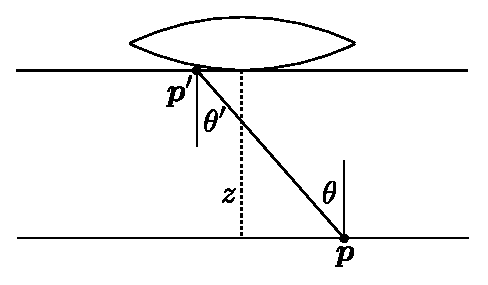
\includegraphics[width=0.5\linewidth]{chap06/Camerameasurementequation.eps}
    \caption{\refeq{6.5}辐射照度度量方程的几何设置。当辐射从
        尾部透镜元件切平面上的点$\bm p'$穿过到胶片平面上的点$\bm p$时可以被度量。
        $z$是从胶片平面到尾部元件切平面的轴向距离\refvar[LensRearZ]{RealisticCamera::LensRearZ}{()},
        而$\theta$是从$\bm p'$到$\bm p$的向量与光轴的夹角。}
    \label{fig:6.25}
\end{figure}

因为胶片平面平行
\sidenote{译者注:原文误写为垂直,已修改。}
于出射瞳平面,所以$\theta=\theta'$。
我们可进一步利用$\bm p$和$\bm p'$间的距离等于从胶片平面到出射瞳轴向距离
(这里我们表示为$z$)除以$\cos\theta$的事实。
将这些全部结合起来,我们有
\begin{align}\label{eq:6.5}
    E({\bm p})=\frac{1}{z^2}\int_{A_{\mathrm{e}}}{L_{\mathrm{i}}({\bm p},{\bm p}')|\cos^4\theta|\mathrm{d}A_{\mathrm{e}}}\, .
\end{align}

对于胶片范围相对于距离$z$较大的相机,项$\cos^4\theta$会
明显降低入射辐射照度——该因素也促成了暗角。
大多数现代数字相机都按照会增加传感器边缘像素值的预设校正因子来校正该效应。

胶片上一点的辐射照度对快门开启时间的积分
给出了\keyindex{注量}{fluence}{}
\sidenote{译者注:即\keyindex{辐射曝光量}{radiant exposure}{}。},
即单位面积上的辐射能量,单位$\text{J/m}^2$。
\begin{align}\label{eq:6.6}
    H({\bm p})=\frac{1}{z^2}\int_{t_0}^{t_1}\int_{A_{\mathrm{e}}}
    L_{\mathrm{i}}({\bm p},{\bm p}',t')|\cos^4\theta|\mathrm{d}A_{\mathrm{e}}\mathrm{d}t'\, .
\end{align}

度量一点的注量刻画了胶片平面接收的能量大小与相机快门开启的时长部分相关的效应。

摄影胶片(或者数字相机内的CCD\sidenote{译者注:即\keyindex{电荷耦合器件}{charge-coupled device}{}。}
或CMOS\sidenote{译者注:即\keyindex{互补式金属氧化物半导体}{complementary metal-oxide-semiconductor}{}。})
实际上是度量一小片面积上的辐射能量
\footnote{2015年代手机数字相机中像素的典型尺寸是每边1.5微米。}。
取\refeq{6.6}并在传感器像素面积$A_{\mathrm{p}}$上积分,我们有
\begin{align}\label{eq:6.7}
    J=\frac{1}{z^2}\int_{A_{\mathrm{p}}}\int_{t_0}^{t_1}\int_{A_{\mathrm{e}}}
    L_{\mathrm{i}}({\bm p},{\bm p}',t')|\cos^4\theta|\mathrm{d}A_{\mathrm{e}}\mathrm{d}t'\mathrm{d}A_{\mathrm{p}}\, ,
\end{align}
焦耳到达一个像素。

\refsec{蒙特卡罗估计器}中,我们将看到蒙特卡罗可以怎样运用于估计这些各种积分的值。
然后\refsub{采样相机1}中我们将定义\refvar{RealisticCamera::GenerateRay}{()}中的
代码片\refcode{Return weighting for RealisticCamera ray}{};
各种计算权重的方法允许我们计算这些量中的每一个。
\refsub{采样相机2}定义了相机模型的\keyindex{重要性函数}{importance function}{},
它表征了其对沿不同光线到达的入射光照的敏感性。

\section{扩展阅读}\label{sec:扩展阅读06}

在他的开创性画板系统中,\citet{10.1145/1461551.1461591}是
第一个为计算机图形学使用投影矩阵的人。
\citet{10.1201/9781315365459}\sidenote{译者注:该书已有第四版\citep{10.1201/b22086}。}给出了
写得非常好的正交和透视投影矩阵的推导。
关于投影的其他优秀参考有\citet{10.5555/63448}的《\citetitle{10.5555/63448}》,
以及\citet{EBERLY2007}关于游戏引擎设计的书籍\sidenote{译者注:原文引用第一版,此处改为引用第二版。}。

\citet{4056910}使用独特的投影方法为Omnimax\textsuperscript{\textregistered}影院
\sidenote{译者注:即现在的IMAX影院。}生成图像。
本章的\refvar{EnvironmentCamera}{}与\citet{KENTON1992288}描述的相机模型相同。

\citet{10.1145/800224.806818,10.1145/357299.357300,10.1145/800059.801169}做了
计算机图形学中景深和运动模糊的早期工作。
Cook和合作者们基于薄透镜模型为这些效应开发了更精确的模型;
它即\refsub{薄透镜模型与景深}中用于景深计算的方法\citep{10.1145/800031.808590,10.1145/7529.8927}。
见\citet{10.2312:EGWR:EGSR07:121-126}关于
具有非针孔光圈的相机可采用的辐射度量类别的广泛分析。

\citet{10.1145/218380.218463}展示了怎样用光线追踪
模拟复杂相机透镜以建模真实相机的成像效应;
\refsec{逼真相机}中的\refvar{RealisticCamera}{}就基于他们的方法。
\citet{10.1111/j.1467-8659.2011.01851.x}改进了该模拟的大量细节,
合并了依赖波长的效应并一起实现衍射和眩光。
\refsub{出射瞳}中我们模拟出射瞳的方法和他们的一样。
见\citet{0321188780}和\citet{9780071476874}的书籍了解
对光学和透镜系统的精彩介绍。

\citet{10.1111/j.1467-8659.2012.03132.x}用多项式来
建模透镜对穿过它们的光线的影响;
它们可以从单个透镜的多项式近似中构造模拟整个透镜系统的多项式。
该方法节约了追踪穿过透镜的光线的计算成本,
不过对于复杂场景其开销相比于剩余的渲染计算量而言一般可以忽略。
\citet{10.1111/cgf.12301}提升了该方法的准确性并展示了怎样将该方法与双向路径追踪结合。

\citet{5280315}介绍了几乎完整模拟数字相机的实现,
包括模数转换\sidenote{译者注:原文analog-to-digital conversion。}和
该过程固有的像素度量值噪声。

\section{习题}\label{sec:习题06}
\begin{enumerate}
      \item \circletwo 一些类型的相机通过在胶片上滑动矩形狭缝
      来曝光胶片。当物体移动方向与曝光狭缝不同时
      会产生有趣效应\citep{761554,10.1080/2151237X.2007.10129235}。
      而且,大多数数字相机在几毫秒时段内从连续扫描线中读出像素值;
      这会造成具有相似视觉特性的\keyindex{卷帘快门}{rolling shutter}{}痕迹。
      在本章的一个或多个相机实现中修改生成时间样本的方式对该效应建模。
      渲染能清楚展示考虑该问题所带来的影响的运动物体图像。
      \item \circletwo 编写一个应用加载由\refvar{EnvironmentCamera}{}渲染的图像,
      并利用纹理映射将其应用在球心位于视点处的球体上,
      使得可以交互地观察它们。用户应能够自由改变观察方向。
      如果为生成球上的纹理坐标使用了正确的纹理映射函数,
      则该应用生成的图像看起来像是观察者处于渲染时相机在场景中的位置,
      因此给予用户交互地环顾场景的能力。
      \item \circletwo \refvar{RealisticCamera}{}中的光圈
      建模为完美的圆;对于可调光圈相机,其光圈通常由
      直边可动叶片构成,因此是$n$边形。修改\refvar{RealisticCamera}{}以
      建模更真实的光圈形状并渲染能展示你模型差异的图像。
      你可能会发现渲染小、亮、失焦物体的场景(例如镜面高光)
      对展示其差异很有用。
      \item \circletwo 计算机图形学中景深的标准模型把
      弥散圆建模为将场景中一点成像为均匀强度的圆盘,
      然而许多真实透镜产生的弥散圆有非线性的变化,例如高斯分布。
      该效应称为\keyindex{散景}{bokeh}{}\citep{10.1145/1242073.1242155}。
      例如,当失焦时观察小光点,反射折射式\sidenote{译者注:原文catadioptric。}(镜面)
      透镜会产生环形高光。修改\refvar{RealisticCamera}{}中
      景深的实现(例如通过偏置透镜样本位置的分布)以生成具有该效应的图像。
      渲染能展示其与标准模型间差异的图像。
      \item \circletwo \keyindex{焦点堆栈渲染}{focal stack rendering}{}:
      焦点堆栈是一固定场景的一系列图像,每张图像的相机对焦距离不同。
      \citet{5740919}与\citet{Jacobs2012}介绍了焦点堆栈的许多应用,
      包括任意的景深,即用户可以指定任意深度对焦,达到传统光学不可能有的效果。
      用pbrt渲染焦点堆栈并编写交互工具以用其控制对焦效应。
      \item \circlethree \keyindex{光场相机}{light field camera}{camera相机}:
      \citet{ng:hal-02551481}讨论了一种相机的物理设计和应用,
      它能捕获胶片上各出射瞳的微小图像,而不是像常规相机那样
      对每一像素在整个出射瞳上的辐射求平均。这样的相机会获取光场的表示——
      到达相机传感器的辐射在空间和方向上变化着的分布。
      通过获取光场,就能实现许多有趣操作,包括拍摄相片后重新对焦。
      阅读\citeauthor{ng:hal-02551481}的论文并在pbrt中实现一个
      获取场景光场的\refvar{Camera}{}。编写工具以允许用户交互地重新对焦这些光场。
      \item \circlethree \refvar{RealisticCamera}{}的实现将胶片置于
      光轴中心并与之垂直。尽管这是真实相机最常见的配置,但通过调整胶片
      相对于透镜系统的放置可以得到有趣的效应。例如,当前实现的焦平面
      总是垂直于光轴;如果胶片平面(或透镜系统)倾斜使得胶片不垂直于光轴,
      则焦平面不再垂直于光轴(这对风景摄影很有用,例如让焦平面
      和地平面对齐时甚至用更大光圈也能有更大景深)。或者可以平移胶片平面
      使得它不在光轴中心;例如可利用该平移保持焦平面和极高物体对齐。
      修改\refvar{RealisticCamera}{}以允许这一或两种调整并渲染展示结果的图像。
      注意当前实现的许多地方(例如出射瞳计算)都有这些修改会违背的假设需要你解决。
\end{enumerate}

{\noindent\hfil$=========$\hfil{\color{red}{施工分割线}}\hfil$=========$\